% ---------------------------------------------------------------------
% --- Arquivo principal (Main_File) do TCC PARKON.
% --- Os demais arquivos sao os dos capitulos e elementos pre/pos-textuais.
% --- Estrutura baseada no template PPGC-UFF-Latex-Abnt (ABNT).
% ---------------------------------------------------------------------

% Configuracao da entrada (opcoes do documento):
%   ruledheader % cabecalho com regua
%   12pt        % tamanho da fonte
%   openright   % capitulos comecam em pagina impar (insere pagina vazia se preciso)
%   a4paper     % tamanho do papel
%   oneside     % impressao apenas no anverso
%   english     % idioma adicional para hifenizacao
%   brazil      % idioma principal do documento (deve ser o ultimo)

\documentclass[ruledheader, 12pt, openright, a4paper, oneside, english, brazil]{PPGC_UFF}


%--- pacotes para hifenizacao e acentuacao em portugues
\usepackage[brazil]{babel}
\usepackage[T1]{fontenc}
\usepackage[utf8]{inputenc}
%\usepackage[latin1]{inputenc}


%--- pacote para figuras
\usepackage{epsf, subfigure}
\usepackage[dvips]{epsfig,graphicx}
\usepackage{chngcntr} %configuracao dos padroes numericos das Figuras e Tabelas
\counterwithout{figure}{chapter} %formata figura para padrao: Figura 1.
\counterwithout{table}{chapter} %formata tabela para padrao: Tabela 1.
\usepackage{float} %permite posicionamento fixo [H] de tabelas/figuras (evita que "flutuem" para longe do titulo)


%--- pacote de simbolos
\usepackage{pifont,textcomp,latexsym}

%--- simbolos matematicos
\usepackage{amssymb,amstext,amsthm,icomma,amsmath}

%--- pacote para gerar pseudo-codigo
\usepackage{algorithm}
\usepackage{algorithmic}
\floatname{algorithm}{Algoritmo}

%--- outros pacotes
\usepackage{url}
\usepackage{longtable}
\usepackage{lscape}
\usepackage{quoting}

%Tabela Colorida
\usepackage{bigdelim,booktabs, colortbl, longtable, multirow, multicol,rotating }


%%===============================================================================
%% INICIO do Pacotes - Lista de abreviaturas, siglas e acronimos
%%===============================================================================
%
% nonumberlist, %do not show page numbers
% acronym,      %generate acronym listing
% nopostdot,    %sem ponto final apos a descricao
% shortcuts,    %habilita atalhos (\acrshort, \acrfull, etc.)
\usepackage[acronym,nopostdot,shortcuts, nonumberlist]{glossaries}


\makeglossaries
% Definições de acrônimos e siglas (glossaries package)
% Fonte: TCC_PARKON_V3.pdf (extraídos do corpo do texto;
% o documento original não possui uma "Lista de Abreviaturas e Siglas" dedicada).
% Formato: \newacronym{<label>}{<sigla>}{<forma por extenso>}
% Ordem alfabética por label.

\newacronym{api}{API}{Application Programming Interface}
\newacronym{apk}{APK}{Android Application Package}
\newacronym{cli}{CLI}{Command Line Interface}
\newacronym{cnpj}{CNPJ}{Cadastro Nacional da Pessoa Jurídica}
\newacronym{cpf}{CPF}{Cadastro de Pessoas Físicas}
\newacronym{rest}{REST}{Representational State Transfer}
\newacronym{rf}{RF}{Requisito Funcional}
\newacronym{rnf}{RNF}{Requisito Não-Funcional}
\newacronym{uff}{UFF}{Universidade Federal Fluminense}
 %definicoes de siglas/acronimos (criado na tarefa 8.1)

%%===============================================================================
%% FIM do Pacotes Lista de abreviaturas, siglas e acronimos
%%===============================================================================

%%===============================================================================
%% Configuracao das citacoes e personalizacao
%%===============================================================================

% Os pacotes abaixo so podem ser usados juntamente com o pacote ABNT abaixo e na ordem atual.
% Esse conjunto de pacotes permite que as citacoes fiquem na cor azul e sejam usadas como link para as referencias.
\usepackage[bookmarksopen=true,
            linktoc=page,
            colorlinks=true,  %ativa a cor do link na referencia
            linkcolor=blue, %muda a cor do link na referencia \ref{} numeros de tabelas, figuras, secoes, sumario etc.
            citecolor=blue, % muda a cor das citacoes \cite \textcite
            filecolor=magenta,
            urlcolor=blue, %muda a cor da url \url no texto e ref. bibliografica
            ]{hyperref}


\usepackage[ %mais informacoes de personalizacao das referencias olhar nos arquivos PDF na pasta MANUAIS
    style = abnt, % Sistema alfabetico
    %style = abnt-numeric, % Sistema numerico
    %style = abnt-ibid, % Notas de referencia
    language=brazil,
    backend=biber,
]{biblatex}

\addbibresource{bibliografia.bib} % A biblioteca de referencias utilizada no trabalho (criada na tarefa 7.1).

%%===============================================================================
%% FIM da configuracao das citacoes e personalizacao
%%===============================================================================

\hyphenation{
a-de-qua-da-men-te
di-men-sio-na-men-to
}

%--------- usando tipo de fonte padrao
% mathptmx (titulos sem negrito) ou ptm (titulos negrito) - Times - Padrao
% ugq (titulos negrito) - Arial
%% -- Padrao do template e: ptm -- %%
\renewcommand{\ABNTchapterfont}{\bfseries\fontfamily{ptm}\fontseries{b}\selectfont}
\renewcommand{\ABNTsectionfont}{\bfseries\fontfamily{ptm}}


% --- -----------------------------------------------------------------
% --- Documento Principal.
% --- -----------------------------------------------------------------

\begin{document}


% --- -----------------------------------------------------------------
% --- Titulo, abstract, dedicatorias e agradecimentos.
% --- Indice geral, lista de figuras e tabelas.
% --- (arquivo na pasta pre-textuais, criado na tarefa 3.x)
% --- -----------------------------------------------------------------
% ---------------------------------------------------------------------
% --- Elementos pre-textuais do TCC PARKON.
% --- Conteudo extraido de TCC_PARKON_V3.pdf (fonte da verdade).
% --- Estrutura baseada no template PPGC-UFF-Latex-Abnt (ABNT).
% ---
% --- NOTA DE ESTRUTURA:
% ---   Este arquivo e construido de forma incremental:
% ---     Tarefa 3.1 (este bloco): capa + folha de rosto + numeracao de paginas
% ---     Tarefa 3.2: termo de aprovacao (sera anexado abaixo)
% ---     Tarefa 3.3: dedicatoria, agradecimentos, resumo e abstract
% ---     Tarefa 3.4: listas (figuras, tabelas, siglas) e sumario
% --- Todo o arquivo deve permanecer em UTF-8.
% ---------------------------------------------------------------------

% --- -----------------------------------------------------------------
% --- Elementos usados na Capa e na Folha de Rosto.
% --- Valores extraidos da capa e folha de rosto de TCC_PARKON_V3.pdf.
% --- -----------------------------------------------------------------
\autor{ANTÔNIO VINICIUS FREITAS FERREIRA} % deve ser escrito em maiusculo

\titulo{Proposta de um Aplicativo para Reserva de Vagas de Estacionamento: Estudo de Caso do Parkon}

\instituicao{UNIVERSIDADE FEDERAL FLUMINENSE}

\orientador{Prof. Dr. Igor Machado Coelho}

% NOTA: A fonte (TCC_PARKON_V3.pdf) nao apresenta coorientador.
% Conforme requisito 3.2, a linha \coorientador foi omitida.

\local{Niterói}

\data{2025} % ano da defesa

% Texto do comentario conforme requisito 3.3 (Curso de Sistemas de Informacao / UFF).
% TODO: [MIGRATION] A area de concentracao nao foi localizada na capa/folha de rosto
%       de TCC_PARKON_V3.pdf. Caso exista, acrescentar ao final do \comentario abaixo
%       no formato: "Área de concentração: <AREA>."
\comentario{Trabalho de Conclusão de Curso apresentado ao Curso de Sistemas de Informação da Universidade Federal Fluminense como requisito parcial para a obtenção do Grau de Bacharel em Sistemas de Informação.}


% --- -----------------------------------------------------------------
% --- Capa. (Capa externa) (Obrigatorio)
% --- -----------------------------------------------------------------
\capa

% --- -----------------------------------------------------------------
% --- Folha de rosto. (Obrigatorio)
% --- -----------------------------------------------------------------
\folhaderosto

% --- -----------------------------------------------------------------
% --- Ficha catalografica (Obrigatoria apenas na versao final de teses/
% --- dissertacoes). A fonte TCC_PARKON_V3.pdf nao contem ficha
% --- catalografica e o arquivo de imagem nao esta disponivel.
% --- TODO: [MIGRATION] Inserir a ficha catalografica aqui caso seja exigida.
% ---       Ex.: \includegraphics em uma figure apontando para
% ---       capitulos/figuras/ficha_catalografica.png
% --- -----------------------------------------------------------------

% --- -----------------------------------------------------------------
% --- Numeracao das paginas pre-textuais em algarismos romanos.
% --- -----------------------------------------------------------------
\pagestyle{ruledheader}
\setcounter{page}{1}
\pagenumbering{roman}

% ---------------------------------------------------------------------
% --- FIM DA TAREFA 3.1 (capa + folha de rosto + numeracao).
% --- O conteudo das tarefas 3.2, 3.3 e 3.4 sera anexado a partir daqui.
% ---------------------------------------------------------------------

% --- -----------------------------------------------------------------
% --- TAREFA 3.2 - Termo de Aprovacao (Folha de Aprovacao). (Obrigatorio)
% --- Conteudo extraido da pagina "Folha de Aprovacao" de TCC_PARKON_V3.pdf.
% --- Banca examinadora (max. 5, incluindo o orientador):
% ---   1) Prof. Dr. Igor Machado Coelho (Orientador) - UFF
% ---   2) Prof. Dr. Raphael Guerra - UFF
% ---   3) Prof. Dr. Joao Felipe Nicolaci Pimentel - UFF
% --- Estrutura espelhada no template PPGC-UFF-Latex-Abnt (layout centrado
% --- com separadores \rule). Arquivo em UTF-8.
% --- -----------------------------------------------------------------
\cleardoublepage
\thispagestyle{empty}

\vspace{-60mm}

\begin{center}
   {\large ANTÔNIO VINICIUS FREITAS FERREIRA}\\
   \vspace{7mm}

   Proposta de um Aplicativo para Reserva de Vagas de Estacionamento: Estudo de Caso do Parkon\\
  \vspace{10mm}
\end{center}

\noindent
\begin{flushright}
\begin{minipage}[t]{8cm}

Trabalho de Conclusão de Curso apresentado ao Curso de Sistemas de Informação da Universidade Federal Fluminense como requisito parcial para a obtenção do Grau de Bacharel em Sistemas de Informação.

\end{minipage}
\end{flushright}
\vspace{1.0 cm}
\noindent
Aprovada em dezembro de 2025. \\
\begin{flushright}
  {
  \begin{center}
  BANCA EXAMINADORA \\
  \vspace{6mm}
  \rule{11cm}{.1mm} \\
    Prof. Dr. Igor Machado Coelho - Orientador, UFF \\
    \vspace{6mm}
  \rule{11cm}{.1mm} \\
    Prof. Dr. Raphael Guerra, UFF \\
    \vspace{6mm}
  \rule{11cm}{.1mm} \\
    Prof. Dr. João Felipe Nicolaci Pimentel, UFF \\
  \vspace{6mm}
  \end{center}
  }
\end{flushright}
\begin{center}
  \vspace{4mm}
  Niterói \\
  2025

\end{center}

% ---------------------------------------------------------------------
% --- FIM DA TAREFA 3.2 (termo de aprovacao).
% --- O conteudo das tarefas 3.3 e 3.4 sera anexado a partir daqui.
% ---------------------------------------------------------------------

% --- -----------------------------------------------------------------
% --- TAREFA 3.3 - Dedicatoria, Agradecimentos, Resumo e Abstract.
% --- Conteudo extraido de TCC_PARKON_V3.pdf (fonte da verdade).
% ---   Pagina 4 -> RESUMO (com Palavras-chave)
% ---   Pagina 5 -> ABSTRACT (com Keywords)
% --- A sequencia de paginas do PDF e: capa -> folha de rosto ->
% --- folha de aprovacao -> RESUMO -> ABSTRACT -> listas.
% --- Arquivo em UTF-8.
% --- -----------------------------------------------------------------

% --- -----------------------------------------------------------------
% --- Dedicatoria. (Opcional - Requisito 3.7, condicional a presenca)
% --- NOTA: [MIGRATION] A fonte TCC_PARKON_V3.pdf NAO contem pagina de
% ---       dedicatoria. Conforme o Requisito 3.7 (condicional a
% ---       presenca da secao no documento de origem), a dedicatoria foi
% ---       OMITIDA. Caso o autor deseje inserir uma dedicatoria, use o
% ---       bloco abaixo (atualmente comentado), que produz um texto em
% ---       italico alinhado a direita em pagina dedicada:
% ---
% --- \cleardoublepage
% --- \thispagestyle{empty}
% --- \vspace*{200mm}
% --- \begin{flushright}
% --- {\em <texto da dedicatoria> }
% --- \end{flushright}
% --- \newpage
% --- -----------------------------------------------------------------

% --- -----------------------------------------------------------------
% --- Agradecimentos. (Opcional - Requisito 3.8, condicional a presenca)
% --- NOTA: [MIGRATION] A fonte TCC_PARKON_V3.pdf NAO contem secao de
% ---       agradecimentos. Conforme o Requisito 3.8 (condicional a
% ---       presenca da secao no documento de origem), os agradecimentos
% ---       foram OMITIDOS. Caso o autor deseje inseri-los, use o bloco
% ---       abaixo (atualmente comentado):
% ---
% --- \pretextualchapter{Agradecimentos}
% --- \hspace{5mm}
% --- <texto dos agradecimentos>
% --- -----------------------------------------------------------------

% --- -----------------------------------------------------------------
% --- Resumo em portugues. (Obrigatorio - Requisito 3.5)
% --- Texto extraido VERBATIM da pagina 4 (RESUMO) de TCC_PARKON_V3.pdf.
% --- Seguido da entrada Palavras-chave em lista rotulada em negrito.
% --- -----------------------------------------------------------------
\begin{resumo}

Este trabalho apresenta o desenvolvimento e a análise do aplicativo móvel Parkon, cujo objetivo é otimizar a busca, reserva e avaliação de vagas de estacionamento em áreas urbanas. O Parkon permite aos usuários localizar vagas disponíveis em tempo real, realizar reservas antecipadas e obter rotas para o estacionamento selecionado. Além disso, oferece um sistema de avaliação da qualidade do serviço e da vaga utilizada, contribuindo para uma experiência mais satisfatória e colaborativa. O desenvolvimento do Parkon foi motivado pela crescente demanda por soluções tecnológicas que reduzam o tempo gasto e aumentem a conveniência no processo de estacionamento, especialmente em grandes centros urbanos. Este estudo descreve as principais funcionalidades do aplicativo, os desafios enfrentados durante sua concepção e as perspectivas para implementação prática.

{\hspace{-8mm} \bf{Palavras-chave}}: Aplicativo móvel, Estacionamento e Reserva de vagas.

\end{resumo}

% --- -----------------------------------------------------------------
% --- Resumo em lingua estrangeira (Abstract). (Obrigatorio - Requisito 3.6)
% --- Texto extraido VERBATIM da pagina 5 (ABSTRACT) de TCC_PARKON_V3.pdf.
% --- Seguido da entrada Keywords em lista rotulada em negrito.
% --- -----------------------------------------------------------------
\begin{abstract}

This work presents the development and analysis of the mobile application Parkon, which aims to optimize the search, reservation, and evaluation of parking spaces in urban areas. Parkon allows users to locate available spaces in real time, make advance reservations, and obtain routes to the selected parking lot. Additionally, it offers a system for evaluating the quality of service and the parking space used, contributing to a more satisfying and collaborative experience. The development of Parkon was motivated by the growing demand for technological solutions that reduce time spent and increase convenience in the parking process, especially in large urban centers. This study describes the main features of the application, the challenges faced during its conception, and the prospects for practical implementation.

{\hspace{-8mm} \bf{Keywords}}: Mobile application, Parking, Space reservation.

\end{abstract}

% ---------------------------------------------------------------------
% --- FIM DA TAREFA 3.3 (dedicatoria, agradecimentos, resumo e abstract).
% --- O conteudo da tarefa 3.4 (listas e sumario) sera anexado a partir daqui.
% ---------------------------------------------------------------------
% --- -----------------------------------------------------------------
% --- TAREFA 3.4 - Listas (figuras, tabelas, siglas) e Sumario.
% --- Estrutura espelhada EXATAMENTE no template PPGC-UFF-Latex-Abnt
% --- (pre-textuais/cap0.tex), respeitando a ordem ABNT e o uso de
% --- \cleardoublepage entre os elementos:
% ---   1) Lista de figuras  (\listoffigures)
% ---   2) Lista de tabelas  (\listoftables)
% ---   3) Lista de abreviaturas e siglas (\printglossary)
% ---   4) Sumario           (\tableofcontents)
% --- Arquivo em UTF-8.
% --- -----------------------------------------------------------------

% --- -----------------------------------------------------------------
% --- Lista de figuras. (Opcional - Requisito 9.3)
% --- -----------------------------------------------------------------
%\cleardoublepage
\listoffigures

% --- -----------------------------------------------------------------
% --- Lista de tabelas. (Opcional - Requisito 9.3)
% --- -----------------------------------------------------------------
\cleardoublepage
\listoftables
\cleardoublepage

% --- -----------------------------------------------------------------
% --- Lista de abreviaturas e siglas. (Opcional - Requisito 7.3)
% --- Elemento que consiste na relacao alfabetica das abreviaturas e
% --- siglas utilizadas no texto, seguidas das expressoes correspondentes
% --- grafadas por extenso (ABNT). Gerada a partir dos acronimos definidos
% --- em pre-textuais/acronimos.tex via pacote glossaries.
% --- -----------------------------------------------------------------
\cleardoublepage
\printglossary[type=\acronymtype,title={Lista de Abreviaturas e Siglas}]
\cleardoublepage

% --- -----------------------------------------------------------------
% --- Sumario. (Obrigatorio - Requisito 9.3)
% --- -----------------------------------------------------------------
\pagestyle{ruledheader}
\tableofcontents
\pagebreak

% ---------------------------------------------------------------------
% --- FIM DA TAREFA 3.4 (listas de figuras, tabelas, siglas e sumario).
% --- Este arquivo pre-textual (cap0.tex) esta COMPLETO.
% ---------------------------------------------------------------------



% --- -----------------------------------------------------------------
% --- Insercao dos capitulos.
% --- Todos os arquivos estao na pasta capitulos.
% --- (capitulos criados nas tarefas 4.1 a 4.5)
% --- -----------------------------------------------------------------

\setcounter{page}{1} %parametros da contagem de paginas.
\pagenumbering{arabic} %padrao de numeros de paginas em arabico (1,2,3)

\pagestyle{ruledheader}
%%%% CAPÍTULO 1 - INTRODUÇÃO
%%
%% Conteúdo extraído VERBATIM de TCC_PARKON_V3.pdf (página 9).
%% Fragmento LaTeX: incluído via \include em tese.tex (sem preâmbulo).
%% Codificação UTF-8.
%%
%% Citações numéricas do original mapeadas para chaves biblatex
%% (padrão {sobrenomePrimeiroAutor}{ano}); serão reconciliadas na tarefa 7.2:
%%   [3] -> \cite{miranda2011}  (MIRANDA, H. F. et al. Mobilidade urbana sustentável e o caso de Curitiba)
%%   [9] -> \cite{wang2011}     (WANG, H. A Reservation-based Smart Parking System)
%% Referências cruzadas a capítulos convertidas para \autoref{} (labels definidos nas tarefas 4.2-4.5).
%% Observação: nenhuma sigla/acrônimo (UFF, API, APK, CLI, RF, RNF) ocorre no texto deste capítulo.

\chapter{Introdução}
\label{cap:introducao}

A crescente urbanização e o aumento da frota de veículos têm intensificado os desafios relacionados à mobilidade urbana~\cite{miranda2011}, especialmente no que se refere à disponibilidade de vagas de estacionamento. Em grandes centros, motoristas enfrentam dificuldades para localizar espaços livres, o que resulta em perda de tempo, aumento do tráfego e maior emissão de poluentes. Nesse cenário, soluções tecnológicas voltadas para otimizar esse processo tornam-se essenciais para melhorar a experiência do usuário e reduzir impactos negativos.

Este trabalho apresenta o desenvolvimento e a análise da plataforma Parkon, cujo objetivo é facilitar a busca, reserva e avaliação de vagas de estacionamento em áreas urbanas. O Parkon é composto por um aplicativo mobile voltado aos motoristas e um portal web administrativo para gestores de estacionamento. O aplicativo permite que os usuários localizem vagas disponíveis em tempo real, realizem reservas antecipadas e recebam rotas para o estacionamento selecionado. Além disso, oferece um sistema de avaliação da qualidade do serviço e da vaga utilizada, promovendo uma experiência mais satisfatória e colaborativa. O portal web permite que administradores cadastrem e gerenciem seus estacionamentos, configurem vagas e acompanhem reservas.

A proposta do Parkon surge da necessidade de reduzir o tempo gasto na procura por vagas e aumentar a conveniência para os motoristas, alinhando-se à tendência de integração entre mobilidade e tecnologia. O desenvolvimento da plataforma foi orientado pela crescente demanda por soluções digitais que otimizem processos cotidianos, especialmente em grandes centros urbanos, onde a falta de vagas é um problema recorrente~\cite{wang2011}.

Este estudo aborda as principais funcionalidades da plataforma, os desafios enfrentados durante sua concepção e as perspectivas para implementação prática. Além disso, discute os benefícios esperados para os usuários e para a mobilidade urbana, considerando aspectos como eficiência, praticidade e sustentabilidade.

O trabalho está estruturado da seguinte forma: o~\autoref{cap:referencial} apresenta o referencial teórico sobre mobilidade urbana e soluções tecnológicas para estacionamento; o~\autoref{cap:proposta} detalha a especificação do sistema, incluindo requisitos e casos de uso; o~\autoref{cap:resultados} apresenta o projeto, protótipo e portal web do sistema; por fim, o~\autoref{cap:conclusao} apresenta as conclusões e sugestões para trabalhos futuros.

% ---------------------------------------------------------------------
% --- CAPITULO 2 - REFERENCIAL TEORICO
% --- Conteudo extraido VERBATIM de TCC_PARKON_V3.pdf (paginas 10-11),
% --- fonte da verdade. Fragmento LaTeX (sem \documentclass/preambulo),
% --- incluido via \include em tese.tex. Arquivo em UTF-8.
% ---
% --- Titulo de origem (corpo do PDF): "REFERENCIAL TEORICO".
% ---   A classe PPGC_UFF formata o titulo do capitulo em maiusculas;
% ---   por isso usa-se \chapter{Referencial Teórico} (mesma saida visivel),
% ---   mantendo a coerencia com o cap1.tex (Requisitos 1.2 e 1.6).
% ---
% --- MAPEAMENTO DE CITACOES (fonte usa numeracao [n]; convertidas para \cite):
% ---   [8]  -> \cite{roche2012}     ROCHE, S. et al. "Are 'Smart Cities' Smart Enough?" (URL: senseable MIT, 2012)
% ---   [4]  -> \cite{antonio2025}   ANTONIO, C. C. Geomarketing e mobilidade urbana (lume.ufrgs)
% ---   [11] -> \cite{estapar2025}   Estapar reserva (site/online)
% ---   [12] -> \cite{parclick2025}  Parclick: Online parking reservation system (site/online)
% ---   TODO: [CITATION] As referencias da fonte NAO trazem ano de publicacao
% ---         explicito (apenas "Acesso em 08 de dez. 2025"). Os anos acima
% ---         sao PROVISORIOS (acesso 2025; roche2012 inferido pela URL) e
% ---         devem ser confirmados/reconciliados nas tarefas 7.1 e 7.2.
% ---
% --- ACRONIMOS usados neste capitulo (definidos em pre-textuais/acronimos.tex):
% ---   api -> primeira ocorrencia no capitulo em 2.3 ("APIs"); usa \acrfullpl{api}
% ---          (forma plural por extenso + sigla). Demais ocorrencias usariam \acrshort.
% ---   NOTA: a reconciliacao da PRIMEIRA ocorrencia entre capitulos sera feita
% ---         na tarefa 10.1 (cross-references).
% ---------------------------------------------------------------------

\chapter{Referencial Teórico}
\label{cap:referencial}

A mobilidade urbana é um dos grandes desafios das cidades modernas \cite{roche2012}, especialmente diante do crescimento acelerado da frota de veículos e da limitação de espaços públicos. O aumento do número de automóveis nas vias resulta em congestionamentos, maior tempo de deslocamento e impactos ambientais, como o aumento da emissão de poluentes. Nesse cenário, torna-se fundamental buscar alternativas que promovam deslocamentos mais eficientes e sustentáveis, integrando tecnologia à infraestrutura urbana para melhorar a qualidade de vida da população.


\section{Mobilidade Urbana e Estacionamento}
\label{sec:mobilidade-estacionamento}

Dentro do contexto da mobilidade urbana, a gestão de vagas de estacionamento representa um dos principais gargalos enfrentados pelos motoristas em grandes centros. A dificuldade em encontrar vagas disponíveis gera perda de tempo, aumenta o fluxo de veículos circulando em busca de espaço e contribui para o agravamento dos congestionamentos. Além disso, esse cenário impacta negativamente a eficiência dos sistemas de transporte e a sustentabilidade das cidades. Soluções tecnológicas voltadas para o monitoramento e reserva de vagas, como aplicativos móveis, surgem como alternativas relevantes para minimizar esses impactos, tornando o processo de estacionamento mais prático, seguro e sustentável.


\section{Aplicativos de Reserva de Vagas}
\label{sec:aplicativos-reserva}

Diversos aplicativos de reserva de vagas \cite{antonio2025} de estacionamento já estão disponíveis no mercado, como Estapar \cite{estapar2025}, Parclick \cite{parclick2025}, Vaga Inteligente e ParkMe. Esses aplicativos oferecem funcionalidades como geolocalização, reserva antecipada, pagamento digital e avaliações de usuários. No entanto, a maioria dessas soluções é voltada exclusivamente para estacionamentos pertencentes à própria companhia desenvolvedora do aplicativo, restringindo o acesso dos usuários apenas à rede de estabelecimentos parceiros ou próprios. Por exemplo, o Estapar permite localizar e reservar vagas apenas em estacionamentos da rede Estapar, enquanto o Vaga Inteligente foca em vagas de condomínios e empresas que aderem à plataforma. O Parclick e o ParkMe também operam com redes específicas, limitando a abrangência e a diversidade de opções para os motoristas. Essa abordagem nichada dificulta a expansão do serviço e reduz a flexibilidade para o usuário, que depende da disponibilidade de vagas apenas nos locais cadastrados pelas empresas.

A proposta do Parkon diferencia-se ao adotar um modelo aberto e colaborativo, semelhante ao conceito do ``iFood'' para restaurantes. Ou seja, qualquer estacionamento pode se cadastrar e gerenciar suas próprias vagas na plataforma, tornando o serviço mais democrático e abrangente. Dessa forma, o Parkon permite que estacionamentos independentes ou de diferentes redes possam se auto-servir, ampliando significativamente as opções para os usuários e promovendo uma experiência mais flexível e inclusiva. Essa abordagem favorece a descentralização do serviço, estimula a concorrência e contribui para a melhoria da mobilidade urbana.


\section{Tecnologias Necessárias}
\label{sec:tecnologias}

O desenvolvimento de aplicativos móveis envolve a integração de diferentes tecnologias e recursos que possibilitam a oferta de serviços eficientes, seguros e acessíveis aos usuários. De modo geral, esses aplicativos dependem de uma arquitetura flexível, capaz de se adaptar a diferentes dispositivos e sistemas operacionais, garantindo uma experiência consistente e intuitiva.

Para que soluções como o Parkon funcionem adequadamente, é fundamental a utilização de tecnologias abertas e padrões amplamente adotados no mercado. Isso inclui, por exemplo, o uso de serviços de geolocalização para identificar a posição do usuário e das vagas disponíveis, integração com sistemas de pagamento digital, mecanismos de autenticação e segurança, além de interfaces que permitam a comunicação entre usuários, estacionamentos e a plataforma central do aplicativo.

Outro ponto importante é a capacidade de atualização em tempo real das informações, permitindo que os usuários tenham acesso imediato à disponibilidade de vagas, avaliações e rotas. A adoção de \acrfullpl{api} abertas e a interoperabilidade entre diferentes sistemas são essenciais para garantir a escalabilidade e a flexibilidade do serviço, possibilitando que novos estacionamentos e funcionalidades sejam incorporados facilmente à plataforma.

Dessa forma, o uso de tecnologias abertas e integradas não só facilita o desenvolvimento e a manutenção do aplicativo, como também amplia o potencial de crescimento e inovação, tornando a solução mais acessível e eficiente para todos os envolvidos.

%%%% CAPÍTULO 3 - ESPECIFICAÇÃO DO SISTEMA
%%
%% Conteúdo extraído VERBATIM de TCC_PARKON_V3.pdf (páginas 12 a 19).
%% Fragmento LaTeX: incluído via \include em tese.tex (sem preâmbulo).
%% Codificação UTF-8.
%%
%% Observações de migração:
%% - Não há citações bibliográficas ([n]) no corpo deste capítulo.
%% - Não há citações diretas com mais de três linhas (nenhum bloco \quoting é necessário).
%% - Não há pseudocódigo/algoritmos neste capítulo (nenhum ambiente \algorithm é necessário).
%% - Referência cruzada "Figura 1" convertida para \autoref{fig:caso-uso-usuario}.
%% - Figuras (Figura 1, 2 e 3): inseridos AMBIENTES PLACEHOLDER com \label para que
%%   os \autoref resolvam; as imagens reais serão extraídas/inseridas na tarefa 5.1.
%% - Tabelas (Tabela 1 a 8): criadas com \label (tab:); estrutura/refino na tarefa 5.2.
%% - Acrônimos: "API" provavelmente já introduzido no Capítulo 2 (seção 2.3 - Tecnologias
%%   Necessárias). Aqui em RNF07 usa-se \acrshortpl{api} (ocorrência subsequente, plural).
%%   A reconciliação de primeiro uso entre capítulos é feita na tarefa 10.1.
%% - Os códigos de requisito "RF01..RF06" e "RNF01..RNF07" são mantidos como
%%   identificadores literais para preservar o conteúdo VERBATIM (Req. 1.1). Os acrônimos
%%   rf/rnf estão definidos em acronimos.tex; sua inclusão na "Lista de Abreviaturas e
%%   Siglas" será tratada nas tarefas 8.1/10.1 (evitar \acrfull aqui alteraria o texto
%%   visível dos códigos).

\chapter{Especificação do Sistema}
\label{cap:proposta}

Considerando que o Parkon é uma plataforma voltada para facilitar a reserva de vagas de estacionamento, sua utilização deve ser intuitiva e acessível para diferentes perfis de usuários. Os requisitos funcionais e não funcionais são fundamentais no desenvolvimento do sistema, pois definem o escopo e a qualidade do produto. Os requisitos funcionais estabelecem as principais funcionalidades que a plataforma deve oferecer, enquanto os requisitos não funcionais determinam critérios de desempenho, segurança e usabilidade. A definição clara desses requisitos é essencial para garantir o sucesso do projeto e a satisfação dos usuários.


\section{Escopo de Utilização}
\label{sec:escopo}

O Parkon foi desenvolvido para facilitar a reserva de vagas de estacionamento em ambientes urbanos. O sistema pode ser utilizado em diferentes cenários, como estacionamentos comerciais, residenciais, públicos ou privados. Os usuários do sistema são divididos em dois perfis: motoristas, que buscam e reservam vagas por meio do aplicativo mobile, e gestores de estacionamento, que cadastram e gerenciam suas vagas e reservas por meio do portal web administrativo.


\section{Análise de Requisitos}
\label{sec:analise-requisitos}

\begin{table}[H]
\begin{center}
\caption{Requisitos Funcionais do Usuário}
\label{tab:requisitos-funcionais}
\begin{tabular}{|c|p{11cm}|}
\hline
\textbf{RF01} & Cadastro de Usuário: Permitir que novos usuários se cadastrem na plataforma, informando dados pessoais e de contato \\
\hline
\textbf{RF02} & Login e Autenticação: Permitir que usuários façam login de forma segura. \\
\hline
\textbf{RF03} & Localização de Vagas: Exibir em tempo real as vagas de estacionamento disponíveis próximas ao usuário, utilizando geolocalização. \\
\hline
\textbf{RF04} & Reserva de Vaga: Permitir que o usuário selecione e reserve uma vaga antecipadamente. \\
\hline
\textbf{RF05} & Avaliação de Vaga/Serviço: Permitir que o usuário avalie a vaga e o serviço após a utilização. \\
\hline
\textbf{RF06} & Geração de Rotas: Fornecer ao usuário a rota até o estacionamento selecionado. \\
\hline
\textbf{RF07} & Responder Comentários: Permitir que o usuário responda a comentários realizados em estacionamentos. \\
\hline
\end{tabular}
\end{center}
\end{table}

\begin{table}[H]
\begin{center}
\caption{Requisitos Funcionais do Administrador do Estacionamento}
\label{tab:requisitos-funcionais-admin}
\begin{tabular}{|c|p{11cm}|}
\hline
\textbf{RF08} & Cadastro do Administrador: Permitir que gestores de estacionamento se cadastrem na plataforma web. \\
\hline
\textbf{RF09} & Login do Administrador: Permitir que o administrador faça login de forma segura no portal web. \\
\hline
\textbf{RF10} & Cadastrar/Editar Empresa: Permitir que o administrador cadastre e edite os dados da empresa responsável pelo estacionamento. \\
\hline
\textbf{RF11} & Cadastrar Estacionamento: Permitir que o administrador cadastre um ou mais estacionamentos vinculados à empresa. \\
\hline
\textbf{RF12} & Configurar Estacionamento: Permitir que o administrador configure informações do estacionamento, como quantidade de vagas, horários de funcionamento e preços. \\
\hline
\textbf{RF13} & Adicionar Colaboradores: Permitir que o administrador adicione outros colaboradores para auxiliar na gestão do estacionamento. \\
\hline
\textbf{RF14} & Visualizar Reservas: Permitir que o administrador visualize as reservas realizadas pelos usuários em seus estacionamentos. \\
\hline
\textbf{RF15} & Confirmar ou Cancelar Reservas: Permitir que o administrador confirme ou cancele reservas de vagas em seus estacionamentos. \\
\hline
\textbf{RF16} & Gerenciar Informações do Estacionamento: Permitir que o administrador atualize informações gerais do estacionamento, como endereço, fotos e descrição. \\
\hline
\end{tabular}
\end{center}
\end{table}

\begin{table}[H]
\begin{center}
\caption{Requisitos Não-Funcionais}
\label{tab:requisitos-nao-funcionais}
\begin{tabular}{|c|p{11cm}|}
\hline
\textbf{RNF01} & Usabilidade: A interface do aplicativo deve ser intuitiva e acessível para usuários de diferentes perfis. \\
\hline
\textbf{RNF02} & Segurança: Os dados dos usuários e transações financeiras devem ser protegidos por mecanismos de autenticação e criptografia. \\
\hline
\textbf{RNF03} & Disponibilidade: O sistema deve estar disponível para acesso 24 horas por dia, 7 dias por semana. \\
\hline
\textbf{RNF04} & Desempenho: As informações sobre vagas disponíveis devem ser atualizadas em tempo real, com tempo de resposta inferior a 2 segundos. \\
\hline
\textbf{RNF05} & Compatibilidade: O aplicativo deve ser compatível com os principais sistemas operacionais móveis (Android e iOS). \\
\hline
\textbf{RNF06} & Escalabilidade: O sistema deve suportar o aumento do número de usuários e estacionamentos cadastrados sem perda de desempenho. \\
\hline
\textbf{RNF07} & Interoperabilidade: O sistema deve permitir integração com \acrshortpl{api} de terceiros, como sistemas de pagamento e mapas. \\
\hline
\end{tabular}
\end{center}
\end{table}


\section{Caso de Uso}
\label{sec:caso-de-uso}

\subsection{Diagramas de Casos de Uso}
\label{sec:diagramas-casos-uso}

Nesta seção, detalhamos os principais eventos que podem ocorrer dentro da plataforma Parkon, considerando os dois atores principais: o usuário motorista, que utiliza o aplicativo mobile para buscar e reservar vagas, e o administrador do estacionamento, que gerencia suas vagas e reservas por meio do portal web administrativo.

Para cada ação realizada pelo usuário, um conjunto de processos é desencadeado, afetando tanto o motorista que faz a reserva quanto o estacionamento que oferece a vaga. O diagrama da \autoref{fig:caso-uso-usuario} representa os casos de uso do usuário do sistema, enquanto o diagrama da \autoref{fig:caso-uso-administrador} apresenta os casos de uso do administrador do estacionamento.

\begin{figure}[H]
   \centering
   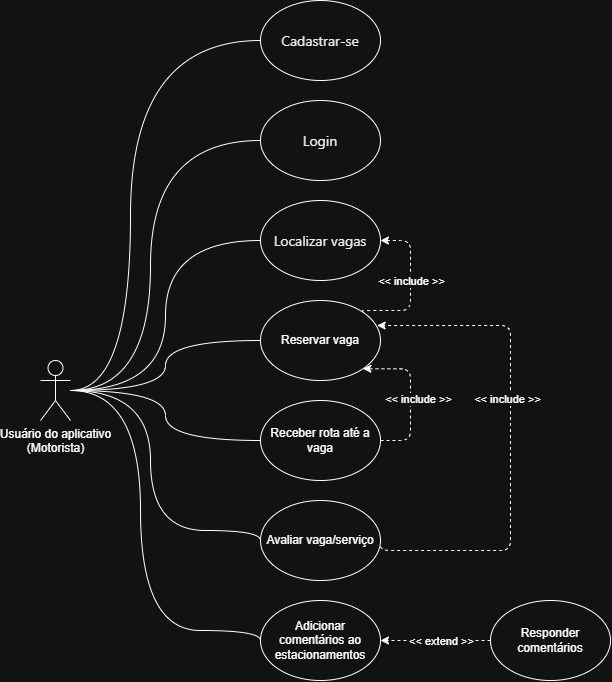
\includegraphics[width=0.6\linewidth]{capitulos/figuras/caso-uso-usuario.png}
   \caption{Diagrama de Caso de Uso do Usuário.}
   \label{fig:caso-uso-usuario}
\end{figure}

\begin{figure}[H]
   \centering
   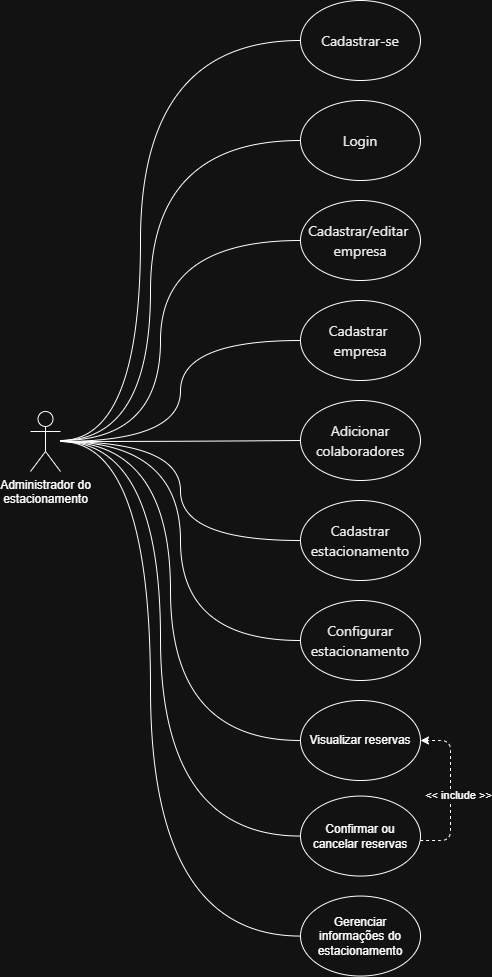
\includegraphics[width=0.6\linewidth]{capitulos/figuras/caso-uso-administrador.png}
   \caption{Diagrama de Caso de Uso do Administrador do Estacionamento.}
   \label{fig:caso-uso-administrador}
\end{figure}


\subsection{Descrição de Casos de Uso}
\label{sec:descricao-casos-uso}

A seguir, descrevemos os principais casos de uso da plataforma Parkon, organizados por ator: o usuário motorista, que utiliza o aplicativo mobile, e o administrador do estacionamento, que gerencia suas operações por meio do portal web.

\subsubsection{Casos de Uso do Usuário (Motorista)}
\label{sec:casos-uso-usuario}

Os casos de uso a seguir descrevem as principais interações do motorista com o aplicativo mobile.

\begin{table}[H]
\begin{center}
\caption{Caso de uso cadastrar-se (Motorista)}
\label{tab:caso-uso-cadastrar}
\begin{tabular}{|p{4cm}|p{9cm}|}
\hline
\textbf{Nome} & Cadastrar-se \\
\hline
\textbf{Objetivos} & Realizar cadastro de usuário na plataforma \\
\hline
\textbf{Atores} & Usuário motorista \\
\hline
\textbf{Pré-Condições} & Não existir cadastro anterior para o mesmo e-mail. \\
\hline
\textbf{Evento Chave (Trigger)} & Abertura do aplicativo pela primeira vez. \\
\hline
\textbf{Fluxo Principal} & 1. Usuário abre o aplicativo. 2. Usuário preenche formulário de cadastro. 3. Usuário clica no botão de cadastrar 4. Usuário é redirecionado para tela de Diálogos. \\
\hline
\textbf{Fluxo Alternativo} & 1. Usuário já está cadastrado. 2. Mensagem para cadastrar com outro e-mail é exibida. \\
\hline
\textbf{Pós-Condições} & Usuário cadastrado no sistema. \\
\hline
\textbf{Regras de Negócios} & Só pode existir um cadastro por e-mail. \\
\hline
\end{tabular}
\end{center}
\end{table}

\begin{table}[H]
\begin{center}
\caption{Caso de uso Login (Motorista)}
\label{tab:caso-uso-login}
\begin{tabular}{|p{4cm}|p{9cm}|}
\hline
\textbf{Nome} & Login \\
\hline
\textbf{Objetivos} & Realizar login na plataforma \\
\hline
\textbf{Atores} & Usuário motorista \\
\hline
\textbf{Pré-Condições} & Ter realizado cadastrado na plataforma anteriormente. \\
\hline
\textbf{Evento Chave (Trigger)} & \\
\hline
\textbf{Fluxo Principal} & 1. Usuário abre o aplicativo. 2. Usuário preenche informações de login. 3. Usuário é redirecionado para tela inícial \\
\hline
\textbf{Fluxo Alternativo} & 1. Usuário não cadastrado. 2. Mensagem para cadastrar é exibida. \\
\hline
\textbf{Pós-Condições} & Usuário autenticado no sistema. \\
\hline
\textbf{Regras de Negócios} & \\
\hline
\end{tabular}
\end{center}
\end{table}

\begin{table}[H]
\begin{center}
\caption{Caso de uso localizar vaga}
\label{tab:caso-uso-localizar-vaga}
\begin{tabular}{|p{4cm}|p{9cm}|}
\hline
\textbf{Nome} & Localizar Vaga \\
\hline
\textbf{Objetivos} & Encontrar estacionamentos na região informada \\
\hline
\textbf{Atores} & Usuário motorista \\
\hline
\textbf{Pré-Condições} & Ter realizado login na plataforma anteriormente. \\
\hline
\textbf{Evento Chave (Trigger)} & Pesquisa do endereço destino \\
\hline
\textbf{Fluxo Principal} & 1. Usuário informa endereço. 2. Usuário recebe lista de estacionamentos. \\
\hline
\textbf{Fluxo Alternativo} & 1. Endereço não encontrado. 2. Mensagem para informar que está incorreto é exibida. \\
\hline
\textbf{Pós-Condições} & \\
\hline
\textbf{Regras de Negócios} & \\
\hline
\end{tabular}
\end{center}
\end{table}

\begin{table}[H]
\begin{center}
\caption{Caso de uso reservar vaga}
\label{tab:caso-uso-reservar-vaga}
\begin{tabular}{|p{4cm}|p{9cm}|}
\hline
\textbf{Nome} & Reservar Vaga \\
\hline
\textbf{Objetivos} & Realizar a reserva de uma vaga no estacionamento selecionado \\
\hline
\textbf{Atores} & Usuário motorista \\
\hline
\textbf{Pré-Condições} & Ter localizado um estacionamento com vagas disponíveis. \\
\hline
\textbf{Evento Chave (Trigger)} & Seleção do estacionamento desejado \\
\hline
\textbf{Fluxo Principal} & 1. Usuário seleciona o estacionamento. 2. Usuário solicita a reserva da vaga. 3. Sistema registra a reserva com status pendente. 4. Administrador do estacionamento confirma a reserva. 5. Usuário é notificado da confirmação. \\
\hline
\textbf{Fluxo Alternativo} & 1. Administrador cancela a reserva. 2. Usuário é notificado do cancelamento. \\
\hline
\textbf{Pós-Condições} & Vaga reservada após aprovação do administrador. \\
\hline
\textbf{Regras de Negócios} & A vaga só é disponibilizada ao usuário após revisão e confirmação do administrador do estacionamento. \\
\hline
\end{tabular}
\end{center}
\end{table}

\begin{table}[H]
\begin{center}
\caption{Caso de uso receber rota até a vaga}
\label{tab:caso-uso-receber-rota}
\begin{tabular}{|p{4cm}|p{9cm}|}
\hline
\textbf{Nome} & Receber rota até a vaga \\
\hline
\textbf{Objetivos} & Obter a rota até o estacionamento encontrado \\
\hline
\textbf{Atores} & Usuário motorista \\
\hline
\textbf{Pré-Condições} & Ter encontrado um estacionamento na busca \\
\hline
\textbf{Evento Chave (Trigger)} & \\
\hline
\textbf{Fluxo Principal} & 1. Usuário encontra estacionamento 2. Sistema abre o google maps no dispositivo do cliente com a rota definida. \\
\hline
\textbf{Fluxo Alternativo} & \\
\hline
\textbf{Pós-Condições} & Usuário com rota definida no google maps \\
\hline
\textbf{Regras de Negócios} & \\
\hline
\end{tabular}
\end{center}
\end{table}

\begin{table}[H]
\begin{center}
\caption{Caso de uso avaliar vaga/serviço}
\label{tab:caso-uso-avaliar}
\begin{tabular}{|p{4cm}|p{9cm}|}
\hline
\textbf{Nome} & Avaliar vaga/serviço \\
\hline
\textbf{Objetivos} & Usuário avaliar a vaga \\
\hline
\textbf{Atores} & Usuário motorista \\
\hline
\textbf{Pré-Condições} & Ter realizado viagem até a vaga \\
\hline
\textbf{Evento Chave (Trigger)} & \\
\hline
\textbf{Fluxo Principal} & 1. Usuário finaliza rota. 2. Usuário realiza avaliação da vaga. \\
\hline
\textbf{Fluxo Alternativo} & \\
\hline
\textbf{Pós-Condições} & Nota do estacionamento é recalculada \\
\hline
\textbf{Regras de Negócios} & \\
\hline
\end{tabular}
\end{center}
\end{table}

\begin{table}[H]
\begin{center}
\caption{Caso de uso adicionar comentários ao estacionamento}
\label{tab:caso-uso-comentarios}
\begin{tabular}{|p{4cm}|p{9cm}|}
\hline
\textbf{Nome} & Adicionar comentários ao estacionamento \\
\hline
\textbf{Objetivos} & Usuário adiciona comentários sobre o estacionamento \\
\hline
\textbf{Atores} & Usuário motorista \\
\hline
\textbf{Pré-Condições} & Estar logado na plataforma \\
\hline
\textbf{Evento Chave (Trigger)} & \\
\hline
\textbf{Fluxo Principal} & 1. Usuário envia comentário do estacionamento. \\
\hline
\textbf{Fluxo Alternativo} & \\
\hline
\textbf{Pós-Condições} & Lista de comentários é atualizada \\
\hline
\textbf{Regras de Negócios} & \\
\hline
\end{tabular}
\end{center}
\end{table}

\begin{table}[H]
\begin{center}
\caption{Caso de uso responder comentários}
\label{tab:caso-uso-responder-comentarios}
\begin{tabular}{|p{4cm}|p{9cm}|}
\hline
\textbf{Nome} & Responder comentários \\
\hline
\textbf{Objetivos} & Permitir que o usuário responda a comentários em estacionamentos \\
\hline
\textbf{Atores} & Usuário motorista \\
\hline
\textbf{Pré-Condições} & Estar logado na plataforma e existir comentários no estacionamento \\
\hline
\textbf{Evento Chave (Trigger)} & Usuário acessa a seção de comentários de um estacionamento \\
\hline
\textbf{Fluxo Principal} & 1. Usuário acessa os comentários do estacionamento. 2. Usuário seleciona um comentário existente. 3. Usuário redige e envia a resposta. \\
\hline
\textbf{Fluxo Alternativo} & \\
\hline
\textbf{Pós-Condições} & Resposta é exibida vinculada ao comentário original \\
\hline
\textbf{Regras de Negócios} & \\
\hline
\end{tabular}
\end{center}
\end{table}

\subsubsection{Casos de Uso do Administrador do Estacionamento}
\label{sec:casos-uso-administrador}

Os casos de uso a seguir descrevem as principais interações do administrador com o portal web administrativo.

\begin{table}[H]
\begin{center}
\caption{Caso de uso cadastrar-se (Administrador)}
\label{tab:caso-uso-cadastrar-admin}
\begin{tabular}{|p{4cm}|p{9cm}|}
\hline
\textbf{Nome} & Cadastrar-se \\
\hline
\textbf{Objetivos} & Realizar cadastro do administrador na plataforma web \\
\hline
\textbf{Atores} & Administrador do estacionamento \\
\hline
\textbf{Pré-Condições} & Não existir cadastro anterior para o mesmo e-mail. \\
\hline
\textbf{Evento Chave (Trigger)} & Acesso ao portal web pela primeira vez \\
\hline
\textbf{Fluxo Principal} & 1. Administrador acessa o portal web. 2. Administrador preenche formulário de cadastro. 3. Administrador confirma o e-mail. 4. Administrador é redirecionado para o painel principal. \\
\hline
\textbf{Fluxo Alternativo} & 1. E-mail já cadastrado. 2. Mensagem informando cadastro existente é exibida. \\
\hline
\textbf{Pós-Condições} & Administrador cadastrado no sistema. \\
\hline
\textbf{Regras de Negócios} & Só pode existir um cadastro por e-mail e por CPF. \\
\hline
\end{tabular}
\end{center}
\end{table}

\begin{table}[H]
\begin{center}
\caption{Caso de uso Login (Administrador)}
\label{tab:caso-uso-login-admin}
\begin{tabular}{|p{4cm}|p{9cm}|}
\hline
\textbf{Nome} & Login \\
\hline
\textbf{Objetivos} & Realizar login no portal web administrativo \\
\hline
\textbf{Atores} & Administrador do estacionamento \\
\hline
\textbf{Pré-Condições} & Ter realizado cadastro na plataforma anteriormente. \\
\hline
\textbf{Evento Chave (Trigger)} & \\
\hline
\textbf{Fluxo Principal} & 1. Administrador acessa o portal web. 2. Administrador preenche informações de login. 3. Administrador é redirecionado para o painel principal. \\
\hline
\textbf{Fluxo Alternativo} & 1. Administrador não cadastrado. 2. Mensagem para cadastrar é exibida. \\
\hline
\textbf{Pós-Condições} & Administrador autenticado no sistema. \\
\hline
\textbf{Regras de Negócios} & \\
\hline
\end{tabular}
\end{center}
\end{table}

\begin{table}[H]
\begin{center}
\caption{Caso de uso cadastrar/editar empresa}
\label{tab:caso-uso-cadastrar-empresa}
\begin{tabular}{|p{4cm}|p{9cm}|}
\hline
\textbf{Nome} & Cadastrar/Editar Empresa \\
\hline
\textbf{Objetivos} & Cadastrar ou editar os dados da empresa responsável pelo estacionamento \\
\hline
\textbf{Atores} & Administrador do estacionamento \\
\hline
\textbf{Pré-Condições} & Estar autenticado no portal web. \\
\hline
\textbf{Evento Chave (Trigger)} & Acesso à seção de empresa no painel \\
\hline
\textbf{Fluxo Principal} & 1. Administrador acessa a seção de empresa. 2. Administrador preenche ou edita os dados (razão social, CNPJ, endereço). 3. Sistema valida e salva as informações. \\
\hline
\textbf{Fluxo Alternativo} & 1. Dados inválidos. 2. Mensagem de erro é exibida solicitando correção. \\
\hline
\textbf{Pós-Condições} & Empresa cadastrada ou atualizada no sistema. \\
\hline
\textbf{Regras de Negócios} & CNPJ deve ser válido e único na plataforma. \\
\hline
\end{tabular}
\end{center}
\end{table}

\begin{table}[H]
\begin{center}
\caption{Caso de uso cadastrar estacionamento}
\label{tab:caso-uso-cadastrar-estacionamento}
\begin{tabular}{|p{4cm}|p{9cm}|}
\hline
\textbf{Nome} & Cadastrar Estacionamento \\
\hline
\textbf{Objetivos} & Cadastrar um novo estacionamento vinculado à empresa \\
\hline
\textbf{Atores} & Administrador do estacionamento \\
\hline
\textbf{Pré-Condições} & Estar autenticado e possuir empresa cadastrada. \\
\hline
\textbf{Evento Chave (Trigger)} & Acesso à seção de estacionamentos no painel \\
\hline
\textbf{Fluxo Principal} & 1. Administrador acessa a seção de estacionamentos. 2. Administrador preenche dados do estacionamento (nome, endereço, capacidade). 3. Sistema valida e cadastra o estacionamento. \\
\hline
\textbf{Fluxo Alternativo} & 1. Endereço já cadastrado por outra empresa. 2. Mensagem informando conflito é exibida. \\
\hline
\textbf{Pós-Condições} & Estacionamento cadastrado e visível para os usuários do aplicativo. \\
\hline
\textbf{Regras de Negócios} & Um estacionamento deve estar vinculado a uma empresa. \\
\hline
\end{tabular}
\end{center}
\end{table}

\begin{table}[H]
\begin{center}
\caption{Caso de uso configurar estacionamento}
\label{tab:caso-uso-configurar-estacionamento}
\begin{tabular}{|p{4cm}|p{9cm}|}
\hline
\textbf{Nome} & Configurar Estacionamento \\
\hline
\textbf{Objetivos} & Definir configurações operacionais do estacionamento \\
\hline
\textbf{Atores} & Administrador do estacionamento \\
\hline
\textbf{Pré-Condições} & Estar autenticado e possuir estacionamento cadastrado. \\
\hline
\textbf{Evento Chave (Trigger)} & Acesso às configurações do estacionamento \\
\hline
\textbf{Fluxo Principal} & 1. Administrador acessa as configurações do estacionamento. 2. Administrador define quantidade de vagas, horários de funcionamento e preços. 3. Sistema salva as configurações. \\
\hline
\textbf{Fluxo Alternativo} & \\
\hline
\textbf{Pós-Condições} & Configurações aplicadas e refletidas no aplicativo mobile. \\
\hline
\textbf{Regras de Negócios} & Quantidade de vagas deve ser maior que zero. \\
\hline
\end{tabular}
\end{center}
\end{table}

\begin{table}[H]
\begin{center}
\caption{Caso de uso adicionar colaboradores}
\label{tab:caso-uso-adicionar-colaboradores}
\begin{tabular}{|p{4cm}|p{9cm}|}
\hline
\textbf{Nome} & Adicionar Colaboradores \\
\hline
\textbf{Objetivos} & Adicionar outros usuários como colaboradores na gestão do estacionamento \\
\hline
\textbf{Atores} & Administrador do estacionamento \\
\hline
\textbf{Pré-Condições} & Estar autenticado e possuir estacionamento cadastrado. \\
\hline
\textbf{Evento Chave (Trigger)} & Acesso à seção de colaboradores \\
\hline
\textbf{Fluxo Principal} & 1. Administrador acessa a seção de colaboradores. 2. Administrador informa o e-mail do colaborador. 3. Sistema envia convite ao colaborador. \\
\hline
\textbf{Fluxo Alternativo} & 1. E-mail não encontrado. 2. Convite é enviado para cadastro na plataforma. \\
\hline
\textbf{Pós-Condições} & Colaborador vinculado ao estacionamento com permissões de gestão. \\
\hline
\textbf{Regras de Negócios} & \\
\hline
\end{tabular}
\end{center}
\end{table}

\begin{table}[H]
\begin{center}
\caption{Caso de uso visualizar reservas}
\label{tab:caso-uso-visualizar-reservas}
\begin{tabular}{|p{4cm}|p{9cm}|}
\hline
\textbf{Nome} & Visualizar Reservas \\
\hline
\textbf{Objetivos} & Visualizar as reservas realizadas pelos usuários \\
\hline
\textbf{Atores} & Administrador do estacionamento \\
\hline
\textbf{Pré-Condições} & Estar autenticado e possuir estacionamento cadastrado. \\
\hline
\textbf{Evento Chave (Trigger)} & Acesso à seção de reservas no painel \\
\hline
\textbf{Fluxo Principal} & 1. Administrador acessa a seção de reservas. 2. Sistema exibe lista de reservas ativas e históricas. \\
\hline
\textbf{Fluxo Alternativo} & 1. Nenhuma reserva encontrada. 2. Mensagem informativa é exibida. \\
\hline
\textbf{Pós-Condições} & \\
\hline
\textbf{Regras de Negócios} & \\
\hline
\end{tabular}
\end{center}
\end{table}

\begin{table}[H]
\begin{center}
\caption{Caso de uso confirmar ou cancelar reservas}
\label{tab:caso-uso-confirmar-cancelar-reservas}
\begin{tabular}{|p{4cm}|p{9cm}|}
\hline
\textbf{Nome} & Confirmar ou Cancelar Reservas \\
\hline
\textbf{Objetivos} & Gerenciar o status das reservas recebidas \\
\hline
\textbf{Atores} & Administrador do estacionamento \\
\hline
\textbf{Pré-Condições} & Existir reserva pendente no estacionamento. \\
\hline
\textbf{Evento Chave (Trigger)} & Nova reserva recebida \\
\hline
\textbf{Fluxo Principal} & 1. Administrador visualiza reserva pendente. 2. Administrador confirma ou cancela a reserva. 3. Sistema notifica o usuário sobre o status. \\
\hline
\textbf{Fluxo Alternativo} & \\
\hline
\textbf{Pós-Condições} & Reserva atualizada e usuário notificado. \\
\hline
\textbf{Regras de Negócios} & Reservas canceladas devem liberar a vaga imediatamente. \\
\hline
\end{tabular}
\end{center}
\end{table}

\begin{table}[H]
\begin{center}
\caption{Caso de uso gerenciar informações do estacionamento}
\label{tab:caso-uso-gerenciar-info}
\begin{tabular}{|p{4cm}|p{9cm}|}
\hline
\textbf{Nome} & Gerenciar Informações do Estacionamento \\
\hline
\textbf{Objetivos} & Atualizar informações gerais do estacionamento \\
\hline
\textbf{Atores} & Administrador do estacionamento \\
\hline
\textbf{Pré-Condições} & Estar autenticado e possuir estacionamento cadastrado. \\
\hline
\textbf{Evento Chave (Trigger)} & Necessidade de atualizar dados do estacionamento \\
\hline
\textbf{Fluxo Principal} & 1. Administrador acessa as informações do estacionamento. 2. Administrador edita dados como endereço, fotos, descrição e contato. 3. Sistema valida e salva as alterações. \\
\hline
\textbf{Fluxo Alternativo} & 1. Dados inválidos. 2. Mensagem de erro é exibida. \\
\hline
\textbf{Pós-Condições} & Informações atualizadas e refletidas no aplicativo mobile. \\
\hline
\textbf{Regras de Negócios} & \\
\hline
\end{tabular}
\end{center}
\end{table}


\section{Modelagem do Sistema}
\label{sec:modelagem-sistema}

\begin{figure}[H]
   \centering
   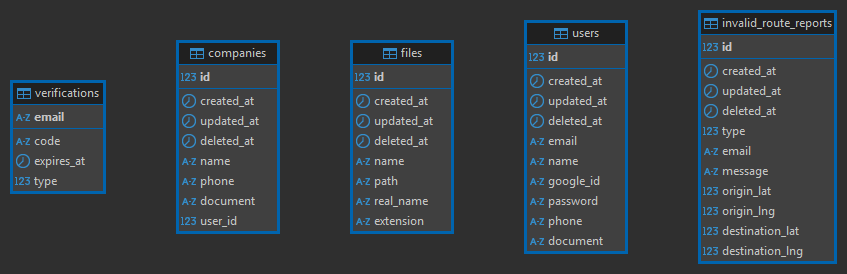
\includegraphics[width=0.95\linewidth]{capitulos/figuras/modelo-classes.png}
   \caption{Modelo de classes utilizado}
   \label{fig:modelo-classes}
\end{figure}

\begin{figure}[H]
   \centering
   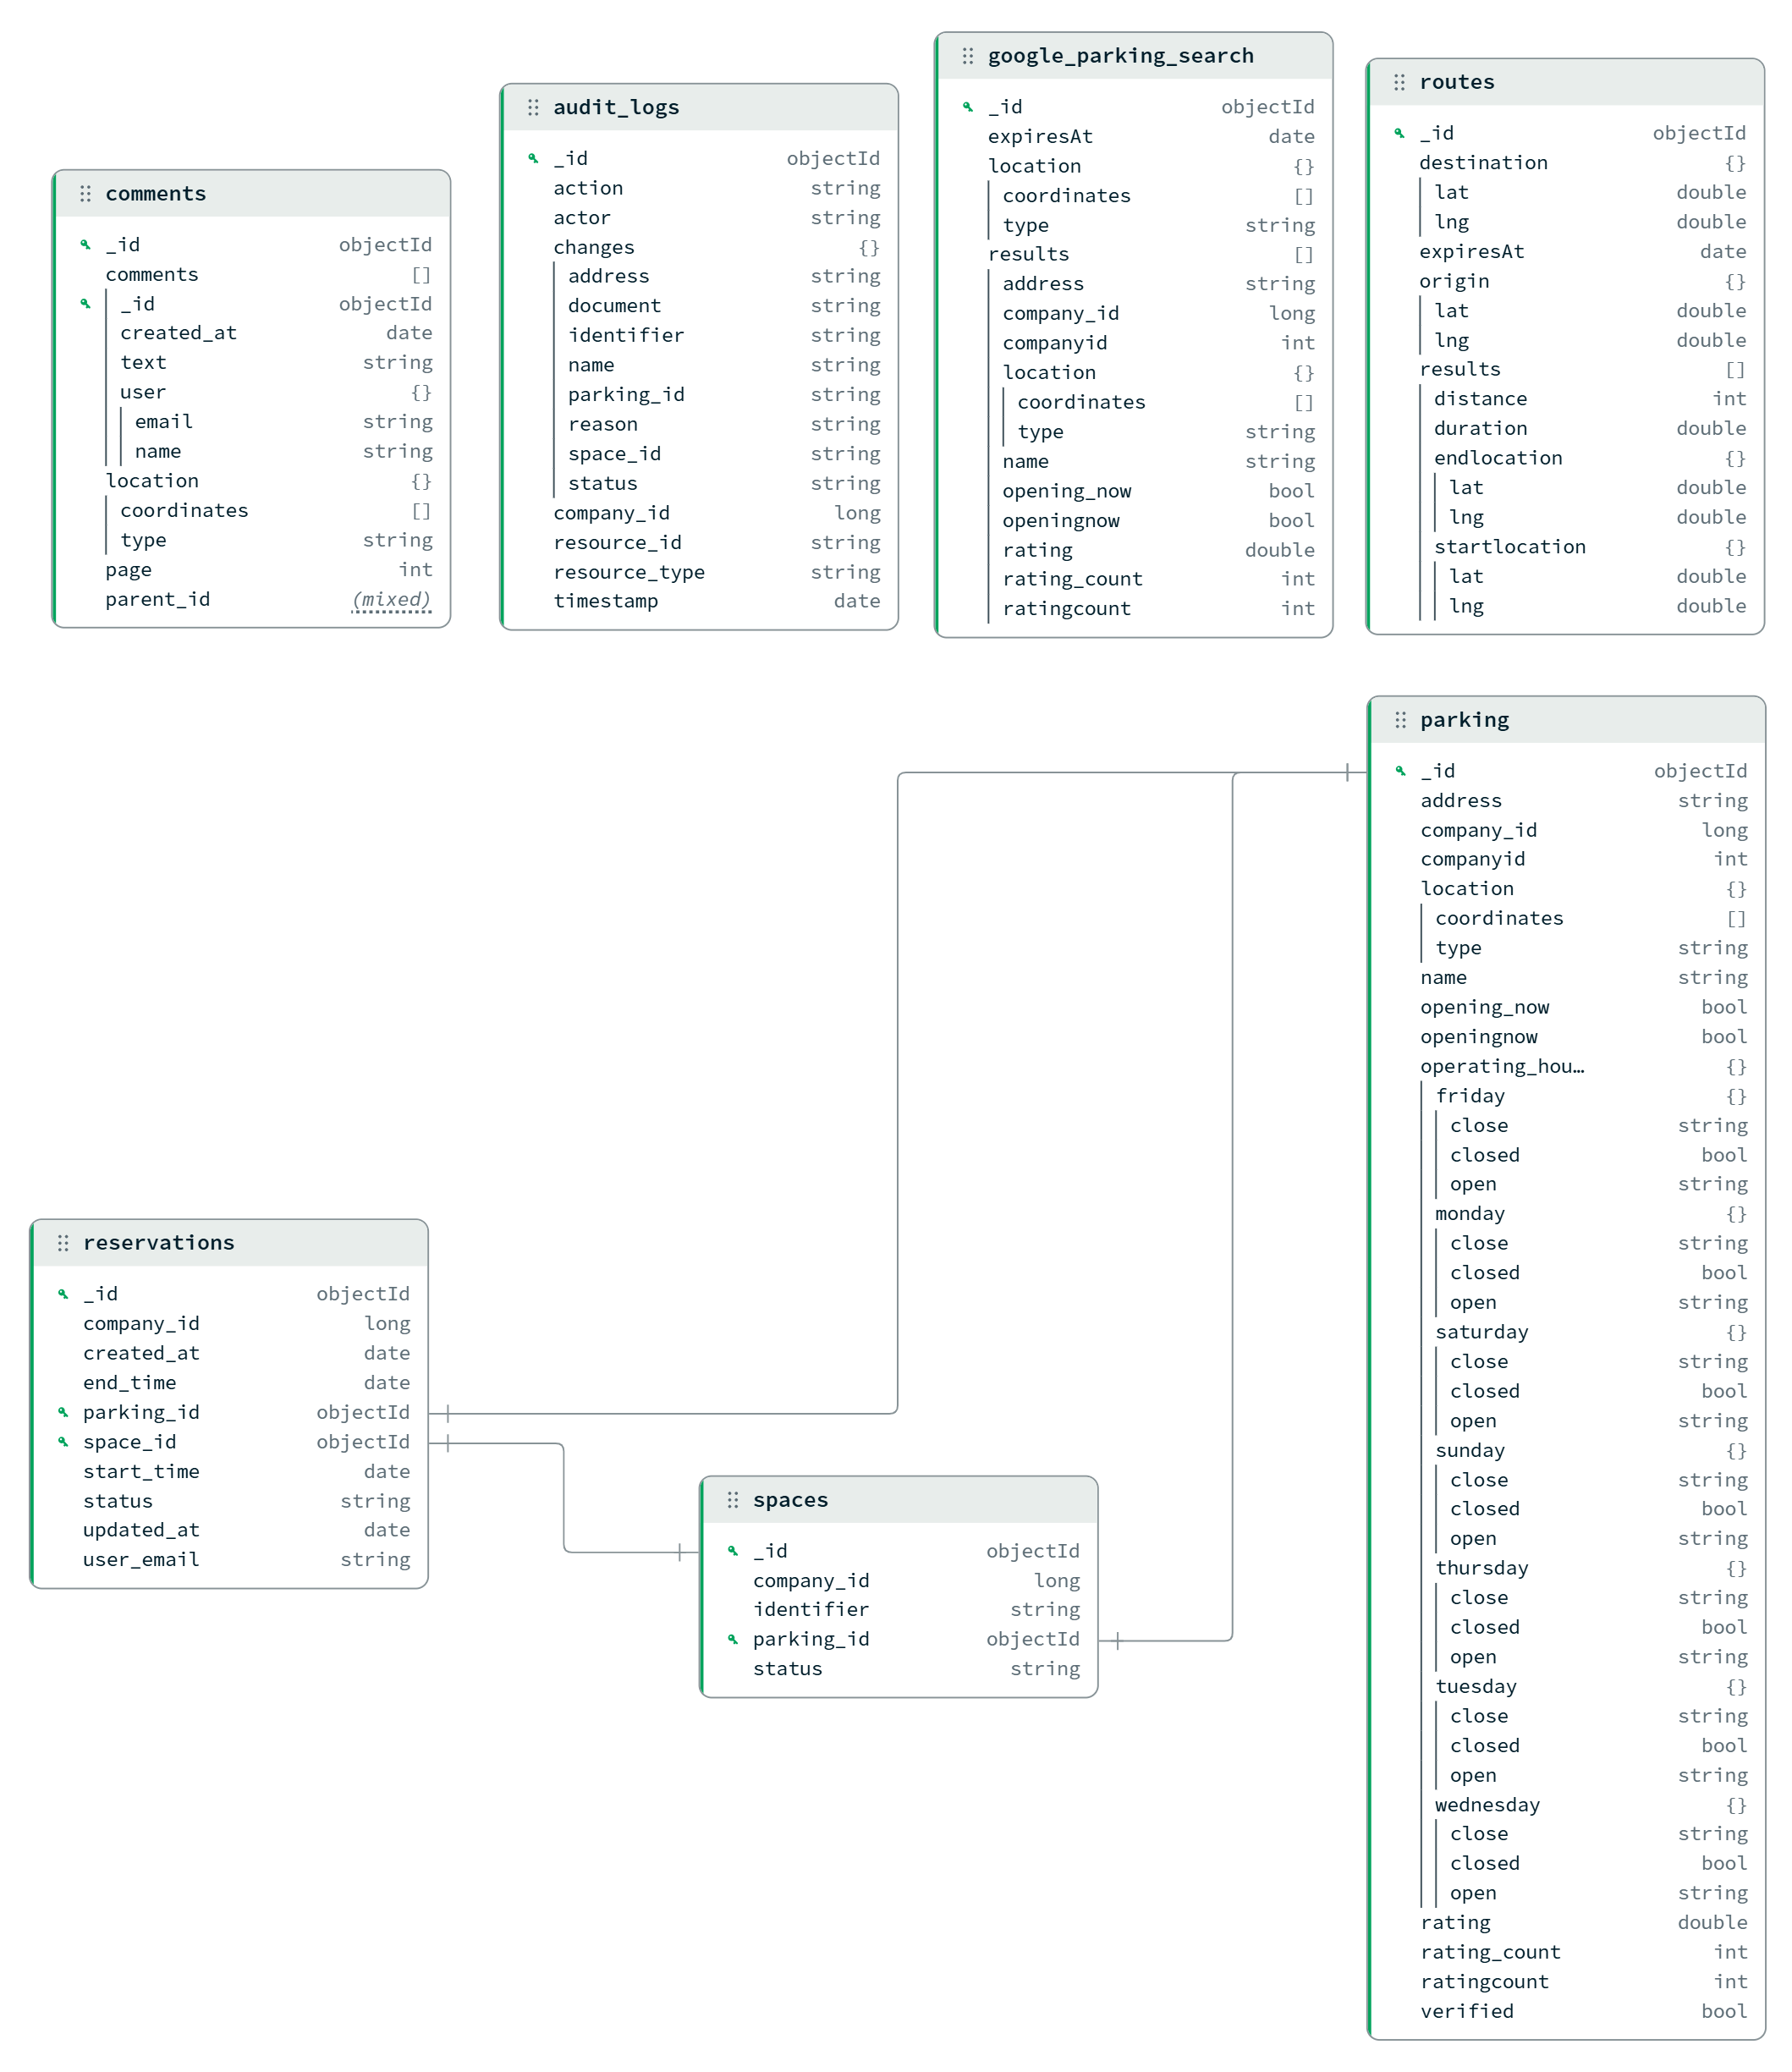
\includegraphics[width=0.95\linewidth]{capitulos/figuras/modelo-mongo.png}
   \caption{Modelo de dados MongoDB}
   \label{fig:modelo-mongo}
\end{figure}

\begin{figure}[H]
   \centering
   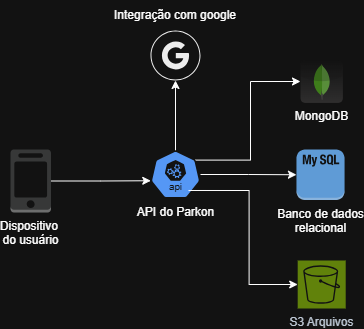
\includegraphics[width=0.55\linewidth]{capitulos/figuras/arquitetura-integracao.png}
   \caption{Arquitetura de integração da aplicação}
   \label{fig:arquitetura-integracao}
\end{figure}

% ---------------------------------------------------------------------
% --- CAPÍTULO 4 - PROJETO E PROTÓTIPO
% ---
% --- Conteúdo extraído VERBATIM de TCC_PARKON_V3.pdf (páginas 20 a 30),
% --- fonte da verdade. Fragmento LaTeX (sem \documentclass/preâmbulo),
% --- incluído via \include em tese.tex. Arquivo em UTF-8.
% ---
% --- Título de origem (corpo do PDF): "4 PROJETO E PROTÓTIPO".
% ---   A classe PPGC_UFF formata o título do capítulo em maiúsculas; por isso
% ---   usa-se \chapter{Projeto e Protótipo} (mesma saída visível), mantendo a
% ---   coerência com os capítulos anteriores (Requisitos 1.2 e 1.6).
% ---   O label é \label{cap:resultados} (referenciado por \autoref{cap:resultados}
% ---   no cap1.tex) conforme definido na tarefa 4.4.
% ---
% --- ESTRUTURA DE SEÇÕES (hierarquia do PDF):
% ---   4   PROJETO E PROTÓTIPO        -> \chapter      (cap:resultados)
% ---   4.1 Criação do protótipo       -> \section      (sec:criacao-prototipo)
% ---   4.2 Criação do projeto         -> \section      (sec:criacao-projeto)
% ---   4.3 Telas do Aplicativo        -> \section      (sec:telas-aplicativo)
% ---   4.4 Build do Aplicativo        -> \section      (sec:build-aplicativo)
% ---
% --- MAPEAMENTO DE CITAÇÕES (fonte usa numeração [n]; convertidas para \cite):
% ---   [7] -> \cite{guarnieri2025}  GUARNIERI, P. L. Estudo de caso comparando o
% ---          MongoDB e o PostgreSQL... (seção 4.2)
% ---   [5] -> \cite{gradin2025}     GRADIN, F. A.; LAZZARETTI, A. T. Um estudo sobre
% ---          o desenvolvimento mobile utilizando Flutter (seção 4.4)
% ---   TODO: [CITATION] As referências da fonte NÃO trazem ano de publicação
% ---         explícito (apenas "Acesso em 08 de dez. 2025"). Os anos acima são
% ---         PROVISÓRIOS (acesso 2025) e devem ser confirmados/reconciliados nas
% ---         tarefas 7.1 e 7.2.
% ---
% --- FIGURAS (Figura 4 a 22): inseridos AMBIENTES PLACEHOLDER com \fbox e \label
% ---   para que os \autoref resolvam; as imagens reais serão extraídas/inseridas
% ---   na tarefa 5.1. Não há tabelas neste capítulo.
% ---
% --- REFERÊNCIAS CRUZADAS: todas as menções "Figura N" no corpo foram convertidas
% ---   para \autoref{fig:...} (Requisito 9.1). Como o template usa
% ---   \counterwithout{figure}{chapter}, a numeração é sequencial no documento;
% ---   o cap3.tex contém as Figuras 1-3, de modo que este capítulo produz
% ---   naturalmente "Figura 4" a "Figura 22", coincidindo com a numeração da fonte.
% ---
% --- ACRÔNIMOS (definidos em pre-textuais/acronimos.tex):
% ---   cli -> ocorre em 4.4 (primeira e única ocorrência da sigla no corpo do
% ---          documento). Na reconciliação de primeiro uso (tarefa 10.1) passou a
% ---          usar \acrfull{cli} (Requisitos 7.2 e 7.5), que renderiza
% ---          "Command Line Interface (CLI)"; removeu-se o parêntese literal
% ---          "(Command Line Interface)" para evitar duplicar a forma por extenso.
% ---   apk -> aparece apenas dentro de um bloco de código/comando verbatim
% ---          ("# Build para Android (APK)"); mantido literal (não convertido),
% ---          por ser conteúdo de linha de comando reproduzido VERBATIM.
% ---
% --- CÓDIGOS/COMANDOS: os blocos de comandos de build (Flutter/Go/Docker) são
% ---   reproduzidos VERBATIM via ambiente \begin{verbatim} (Requisito 1.1).
% ---------------------------------------------------------------------

\chapter{Projeto e Protótipo}
\label{cap:resultados}

\section{Criação do protótipo}
\label{sec:criacao-prototipo}

O protótipo do aplicativo Parkon foi desenvolvido com o objetivo de validar as principais funcionalidades propostas para a reserva de vagas de estacionamento em ambientes urbanos. Utilizando ferramentas de prototipagem, foram criadas telas que simulam a experiência do usuário, permitindo a visualização do fluxo de navegação, das opções de busca e reserva de vagas, bem como dos mecanismos de avaliação e pagamento. O protótipo serve como base para testes iniciais de usabilidade e para o refinamento dos requisitos do sistema, antes da implementação definitiva.

\begin{figure}[H]
   \centering
   \begin{minipage}[b]{0.48\linewidth}
      \centering
      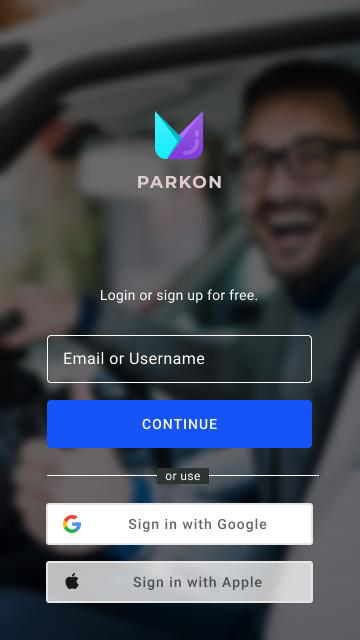
\includegraphics[height=0.34\textheight,keepaspectratio]{capitulos/figuras/tela-autenticacao.png}
      \caption{Tela de Autenticação}
      \label{fig:tela-autenticacao}
   \end{minipage}\hfill
   \begin{minipage}[b]{0.48\linewidth}
      \centering
      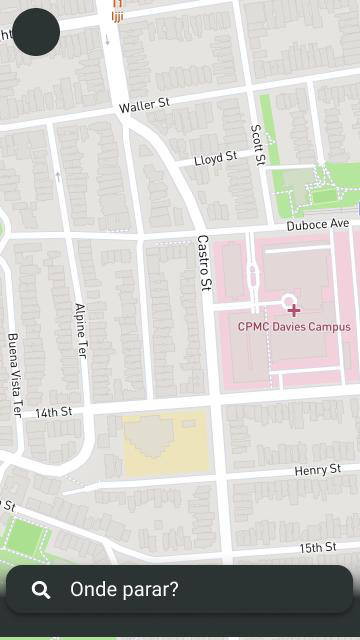
\includegraphics[height=0.34\textheight,keepaspectratio]{capitulos/figuras/tela-inicial.png}
      \caption{Tela Inicial do aplicativo}
      \label{fig:tela-inicial}
   \end{minipage}
\end{figure}

A \autoref{fig:tela-autenticacao} apresenta a tela de autenticação do aplicativo Parkon, onde o usuário pode realizar login ou cadastro, inclusive utilizando contas do Google ou Apple, em uma interface simples e moderna. Já a \autoref{fig:tela-inicial} mostra a tela inicial, composta por um mapa interativo e um campo de pesquisa ``Onde parar?'', permitindo ao usuário localizar estacionamentos próximos de forma prática e eficiente.

\begin{figure}[H]
   \centering
   \begin{minipage}[b]{0.48\linewidth}
      \centering
      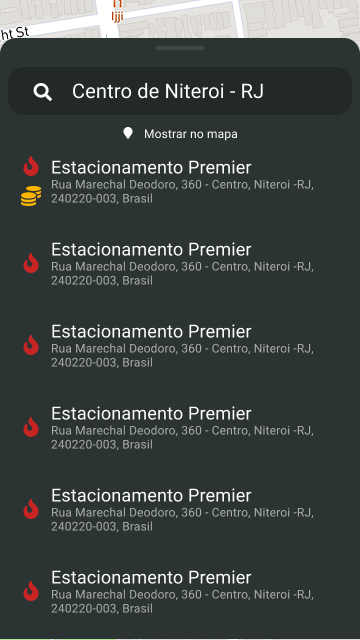
\includegraphics[height=0.34\textheight,keepaspectratio]{capitulos/figuras/tela-pesquisa-vagas.png}
      \caption{Tela de Pesquisa de Vagas}
      \label{fig:tela-pesquisa-vagas}
   \end{minipage}\hfill
   \begin{minipage}[b]{0.48\linewidth}
      \centering
      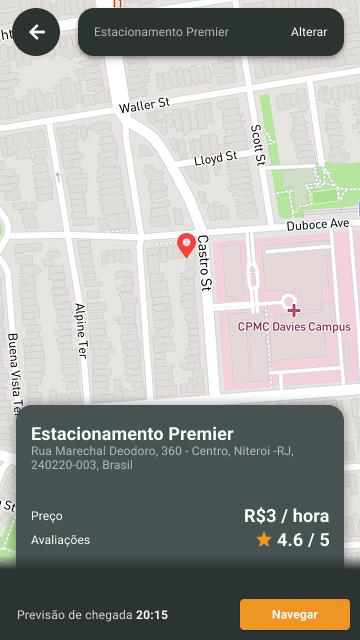
\includegraphics[height=0.34\textheight,keepaspectratio]{capitulos/figuras/tela-selecao-estacionamento.png}
      \caption{Tela de Seleção de Estacionamento}
      \label{fig:tela-selecao-estacionamento}
   \end{minipage}
\end{figure}

A \autoref{fig:tela-pesquisa-vagas} apresenta a tela de pesquisa de vagas do aplicativo Parkon, onde o usuário pode inserir o destino desejado e visualizar uma lista de estacionamentos disponíveis na região, facilitando a escolha do local para estacionar. Já a \autoref{fig:tela-selecao-estacionamento} mostra a tela de seleção de estacionamento, exibindo detalhes como endereço, preço, avaliações e previsão de chegada, além de permitir ao usuário navegar até o estacionamento escolhido.

\begin{figure}[H]
   \centering
   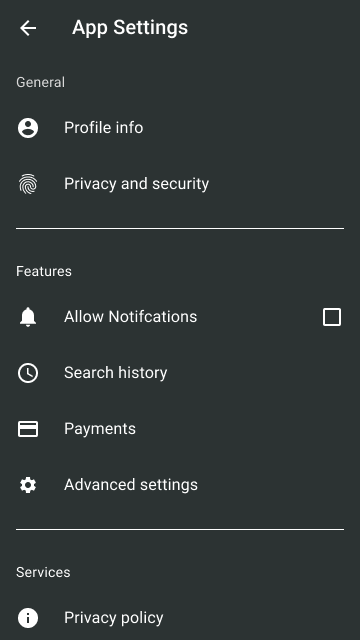
\includegraphics[height=0.42\textheight,keepaspectratio]{capitulos/figuras/tela-configuracoes.png}
   \caption{Tela de Configurações}
   \label{fig:tela-configuracoes}
\end{figure}

\section{Criação do projeto}
\label{sec:criacao-projeto}

\subsection{Aplicativo Mobile (Flutter)}
\label{sec:criacao-projeto-mobile}

O desenvolvimento do projeto do aplicativo Parkon foi realizado utilizando o framework Flutter, escolhido por sua capacidade de criar aplicações móveis multiplataforma com uma única base de código, facilitando a manutenção e a escalabilidade do sistema. Durante a implementação, um dos principais desafios enfrentados foi a integração do serviço de geolocalização do Google, essencial para identificar a localização do usuário e das vagas disponíveis em tempo real. Para garantir o desempenho e a disponibilidade das informações, foi adotado um mecanismo de cache utilizando o banco de dados MongoDB~\cite{guarnieri2025}, permitindo o armazenamento temporário dos dados de localização e otimizando o acesso mesmo em situações de instabilidade de conexão. Essa abordagem proporcionou maior eficiência ao aplicativo, reduzindo o tempo de resposta e melhorando a experiência do usuário.

\subsection{Portal Web Administrativo (Next.js)}
\label{sec:criacao-projeto-web}

O portal web administrativo foi desenvolvido utilizando React com o framework Next.js, permitindo que gestores de estacionamento realizem operações de cadastro, configuração e acompanhamento de reservas por meio de uma interface web responsiva.

A escolha do Next.js se deu pela facilidade de integração com a \acrshort{api} REST já existente no backend em Go, além de oferecer renderização do lado do servidor, o que proporciona melhor desempenho no carregamento inicial das páginas. A interface foi construída com componentes reutilizáveis, seguindo padrões de design responsivo para garantir acessibilidade em diferentes dispositivos.

O portal compartilha a mesma infraestrutura de backend e banco de dados (MongoDB) utilizada pelo aplicativo mobile, garantindo consistência dos dados entre ambas as plataformas. A autenticação é realizada por meio do mesmo serviço de autenticação, permitindo que as credenciais do administrador sejam utilizadas de forma unificada.

\section{Telas do Aplicativo}
\label{sec:telas-aplicativo}

\subsection{Telas do Aplicativo Mobile}
\label{sec:telas-mobile}

\begin{figure}[H]
   \centering
   \begin{minipage}[b]{0.48\linewidth}
      \centering
      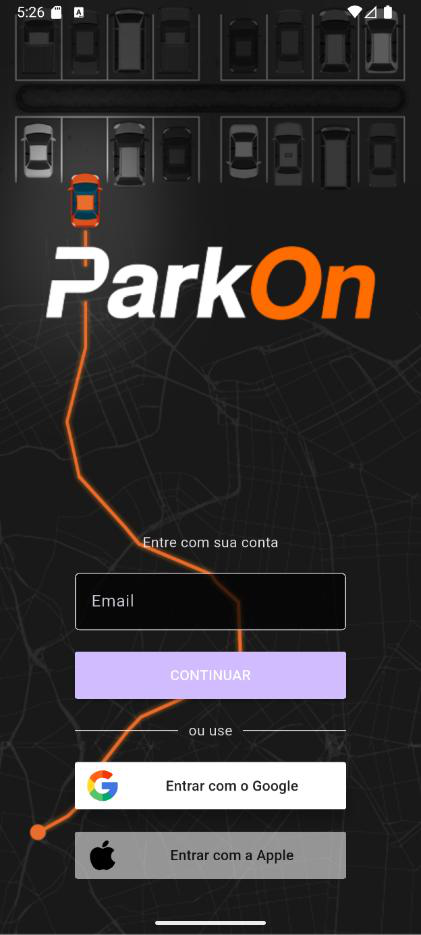
\includegraphics[height=0.34\textheight,keepaspectratio]{capitulos/figuras/emulador-login.png}
      \caption{Aplicação rodando no emulador - Login}
      \label{fig:emulador-login}
   \end{minipage}\hfill
   \begin{minipage}[b]{0.48\linewidth}
      \centering
      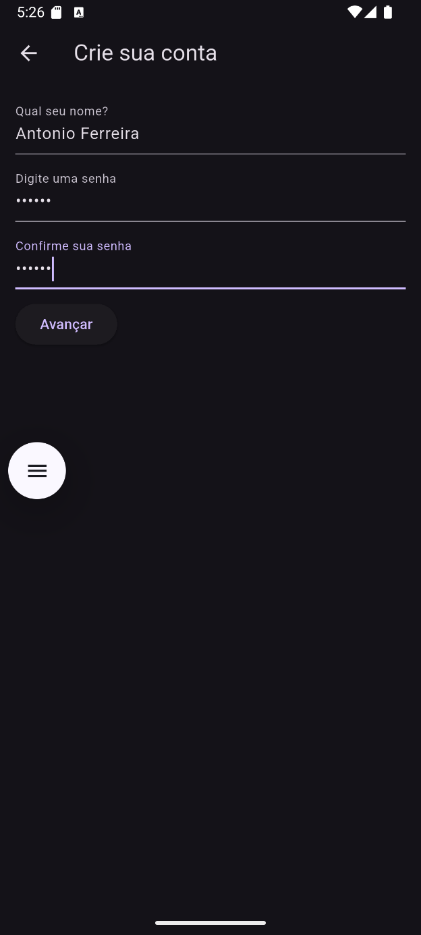
\includegraphics[height=0.34\textheight,keepaspectratio]{capitulos/figuras/emulador-cadastro.png}
      \caption{Aplicação rodando no emulador - Cadastro}
      \label{fig:emulador-cadastro}
   \end{minipage}
\end{figure}

A \autoref{fig:emulador-login} mostra a tela de login do aplicativo Parkon em funcionamento no emulador, destacando o campo para inserção de e-mail e opções de autenticação, incluindo Google e Apple, em um layout moderno e funcional. A \autoref{fig:emulador-cadastro} apresenta a tela de cadastro, onde o usuário informa nome e senha para criar sua conta.

\begin{figure}[H]
   \centering
   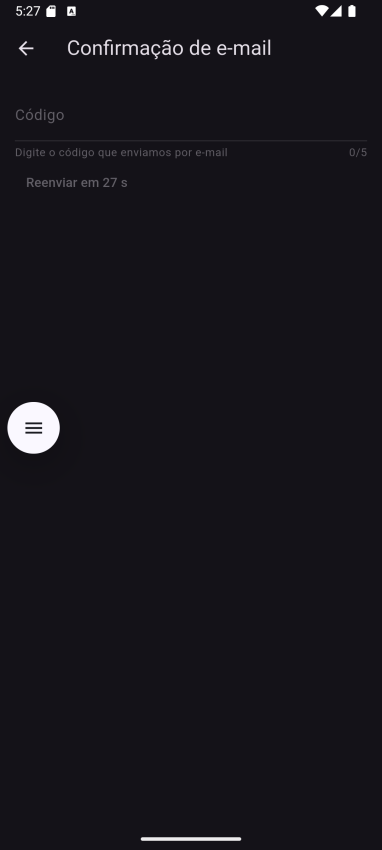
\includegraphics[height=0.34\textheight,keepaspectratio]{capitulos/figuras/emulador-confirmacao-email.png}
   \caption{Aplicação rodando no emulador - Confirmação de e-mail}
   \label{fig:emulador-confirmacao-email}

   \vspace{0.6cm}

   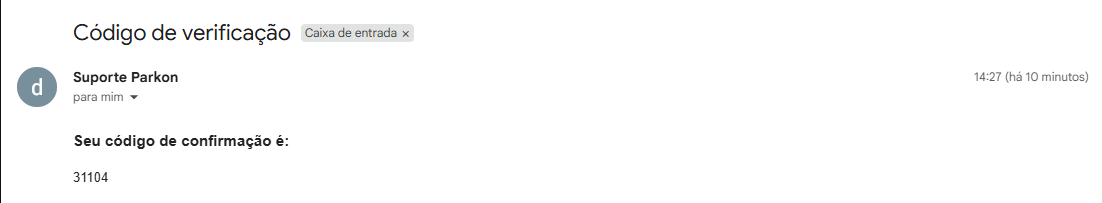
\includegraphics[width=0.85\linewidth]{capitulos/figuras/emulador-email-codigo.png}
   \caption{Aplicação rodando no emulador – E-mail com o código}
   \label{fig:emulador-email-codigo}
\end{figure}

A \autoref{fig:emulador-confirmacao-email} apresenta a tela de confirmação de e-mail do aplicativo Parkon, onde o usuário deve inserir o código recebido para validar o cadastro. Já a \autoref{fig:emulador-email-codigo} mostra o e-mail enviado ao usuário com o código de verificação necessário para concluir o processo de registro.

\begin{figure}[H]
   \centering
   \begin{minipage}[b]{0.48\linewidth}
      \centering
      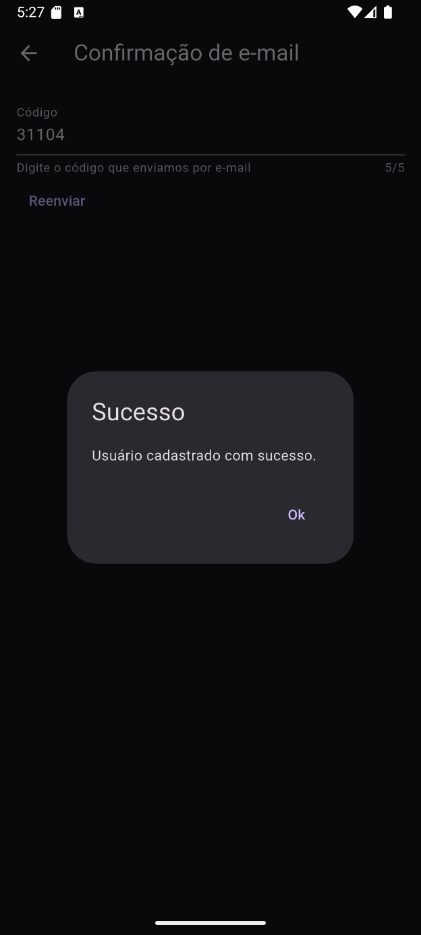
\includegraphics[height=0.34\textheight,keepaspectratio]{capitulos/figuras/emulador-sucesso-cadastro.png}
      \caption{Aplicação rodando no emulador - Sucesso no cadastro}
      \label{fig:emulador-sucesso-cadastro}
   \end{minipage}\hfill
   \begin{minipage}[b]{0.48\linewidth}
      \centering
      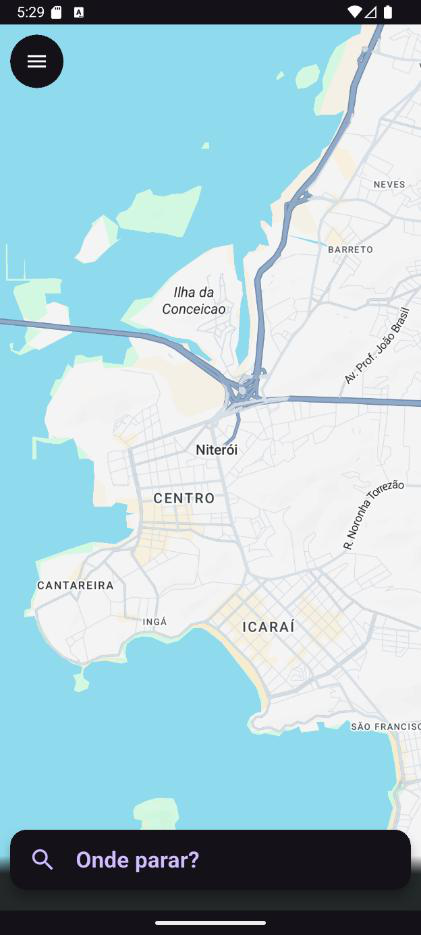
\includegraphics[height=0.34\textheight,keepaspectratio]{capitulos/figuras/emulador-tela-inicial.png}
      \caption{Aplicação rodando no emulador – Tela ínicial}
      \label{fig:emulador-tela-inicial}
   \end{minipage}
\end{figure}

A \autoref{fig:emulador-sucesso-cadastro} mostra a tela de confirmação de sucesso no cadastro do usuário, indicando que o processo foi concluído corretamente no aplicativo Parkon. Já a \autoref{fig:emulador-tela-inicial} apresenta a tela inicial do aplicativo após o login, exibindo o mapa da região e o campo de pesquisa para localização de vagas.

\begin{figure}[H]
   \centering
   \begin{minipage}[b]{0.48\linewidth}
      \centering
      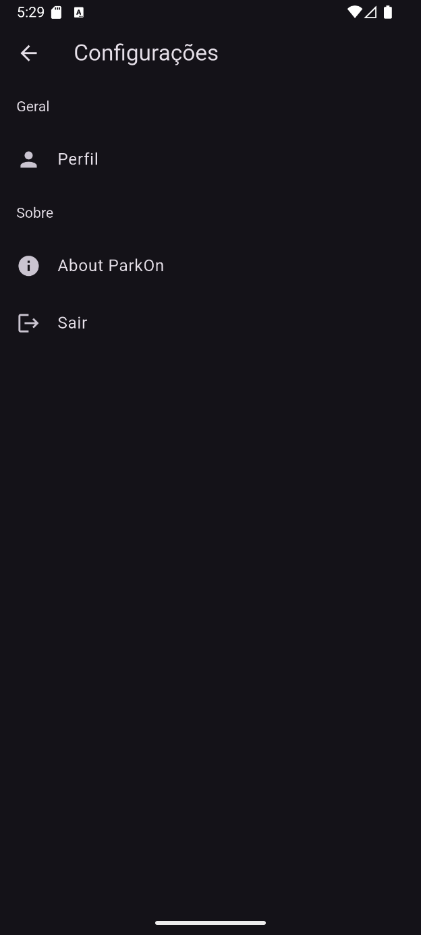
\includegraphics[height=0.34\textheight,keepaspectratio]{capitulos/figuras/emulador-configuracoes.png}
      \caption{Aplicação rodando no emulador - Configurações}
      \label{fig:emulador-configuracoes}
   \end{minipage}\hfill
   \begin{minipage}[b]{0.48\linewidth}
      \centering
      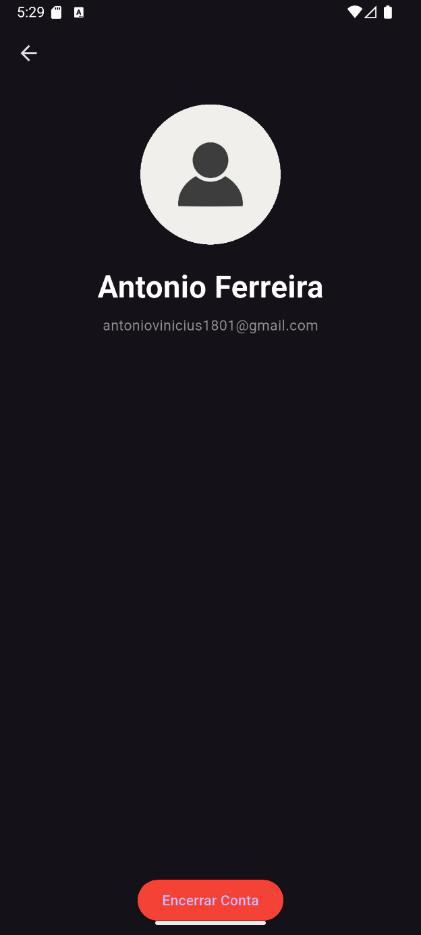
\includegraphics[height=0.34\textheight,keepaspectratio]{capitulos/figuras/emulador-perfil.png}
      \caption{Aplicação rodando no emulador – Perfil do usuário}
      \label{fig:emulador-perfil}
   \end{minipage}
\end{figure}

A \autoref{fig:emulador-configuracoes} apresenta a tela de configurações do aplicativo Parkon, onde o usuário pode acessar opções como perfil, privacidade, histórico de buscas, pagamentos e ajustes gerais. A \autoref{fig:emulador-perfil} mostra a tela de perfil do usuário, exibindo dados pessoais e a opção de encerrar a conta.

\begin{figure}[H]
   \centering
   \begin{minipage}[b]{0.48\linewidth}
      \centering
      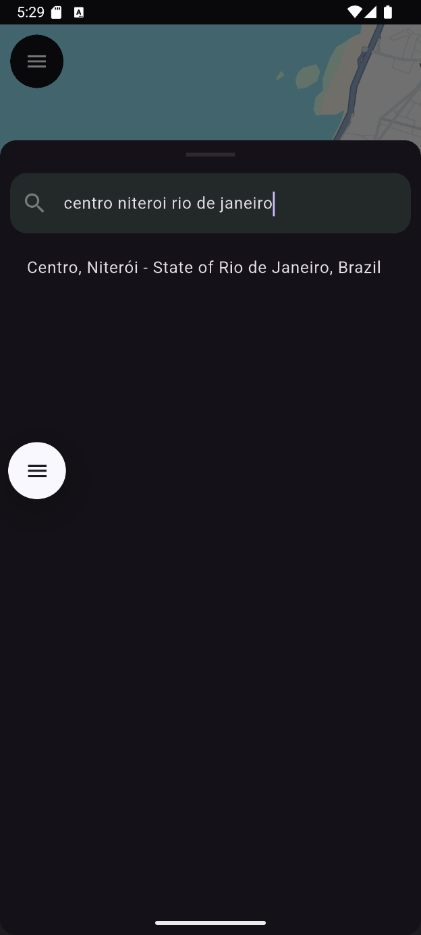
\includegraphics[height=0.34\textheight,keepaspectratio]{capitulos/figuras/emulador-pesquisa.png}
      \caption{Aplicação rodando no emulador - Pesquisa de estacionamento}
      \label{fig:emulador-pesquisa}
   \end{minipage}\hfill
   \begin{minipage}[b]{0.48\linewidth}
      \centering
      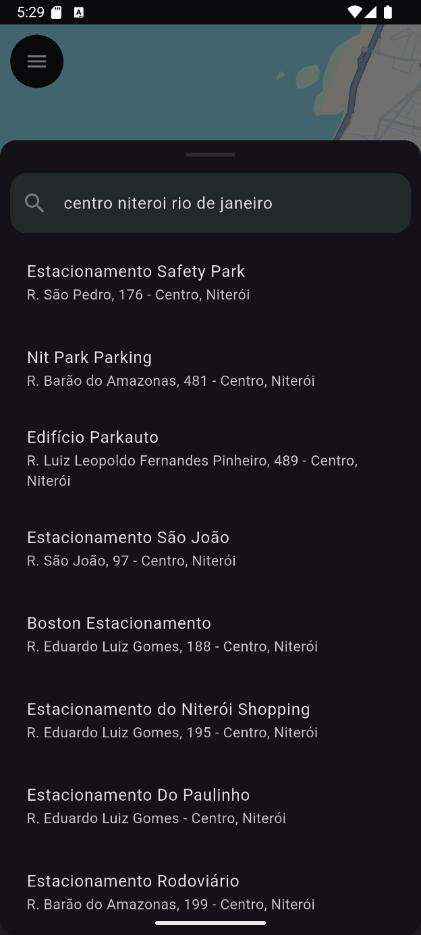
\includegraphics[height=0.34\textheight,keepaspectratio]{capitulos/figuras/emulador-lista.png}
      \caption{Aplicação rodando no emulador - Lista de estacionamentos}
      \label{fig:emulador-lista}
   \end{minipage}
\end{figure}

A \autoref{fig:emulador-pesquisa} apresenta a tela de pesquisa de estacionamento do aplicativo Parkon, onde o usuário pode digitar o endereço desejado para localizar vagas disponíveis na região. A \autoref{fig:emulador-lista} mostra a lista de estacionamentos encontrados, exibindo opções próximas ao destino informado pelo usuário.

\begin{figure}[H]
   \centering
   \begin{minipage}[b]{0.48\linewidth}
      \centering
      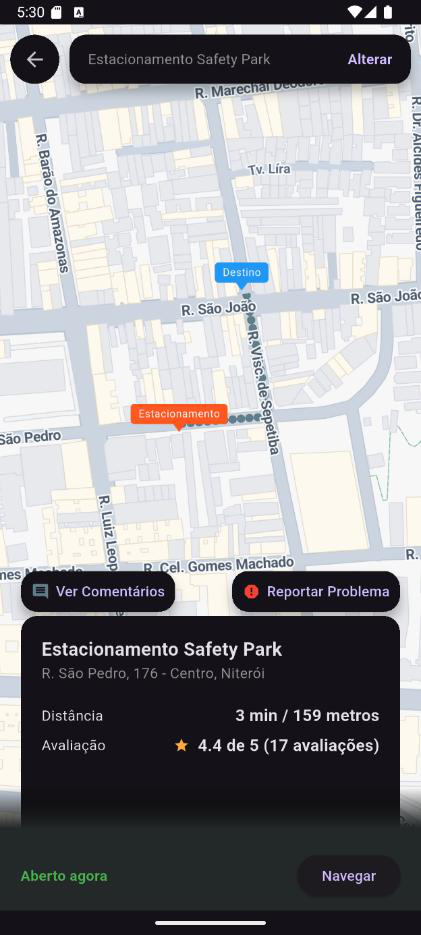
\includegraphics[height=0.34\textheight,keepaspectratio]{capitulos/figuras/emulador-detalhes.png}
      \caption{Aplicação rodando no emulador - Detalhes do estacionamento}
      \label{fig:emulador-detalhes}
   \end{minipage}\hfill
   \begin{minipage}[b]{0.48\linewidth}
      \centering
      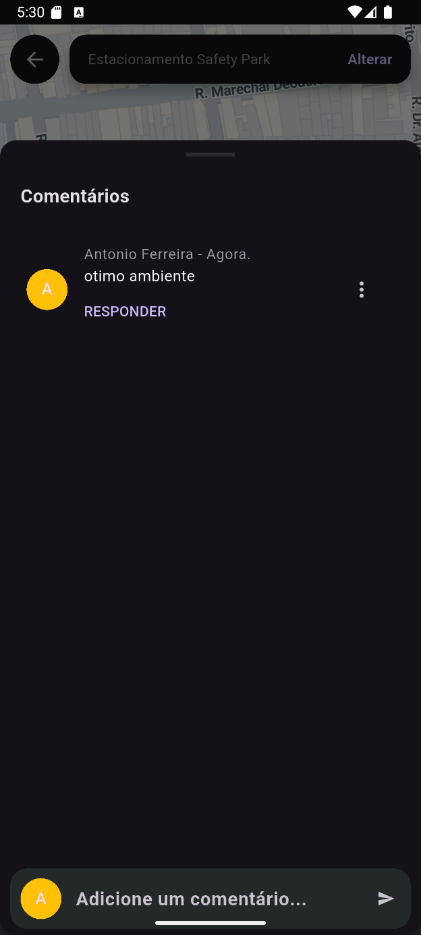
\includegraphics[height=0.34\textheight,keepaspectratio]{capitulos/figuras/emulador-comentarios.png}
      \caption{Aplicação rodando no emulador - Comentários}
      \label{fig:emulador-comentarios}
   \end{minipage}
\end{figure}

A \autoref{fig:emulador-detalhes} mostra a tela de detalhes do estacionamento no aplicativo Parkon, exibindo informações como endereço, distância, avaliações e opções para ver comentários ou reportar problemas. A \autoref{fig:emulador-comentarios} apresenta a tela de comentários, onde o usuário pode visualizar e adicionar opiniões sobre o estacionamento selecionado.

\begin{figure}[H]
   \centering
   \begin{minipage}[b]{0.48\linewidth}
      \centering
      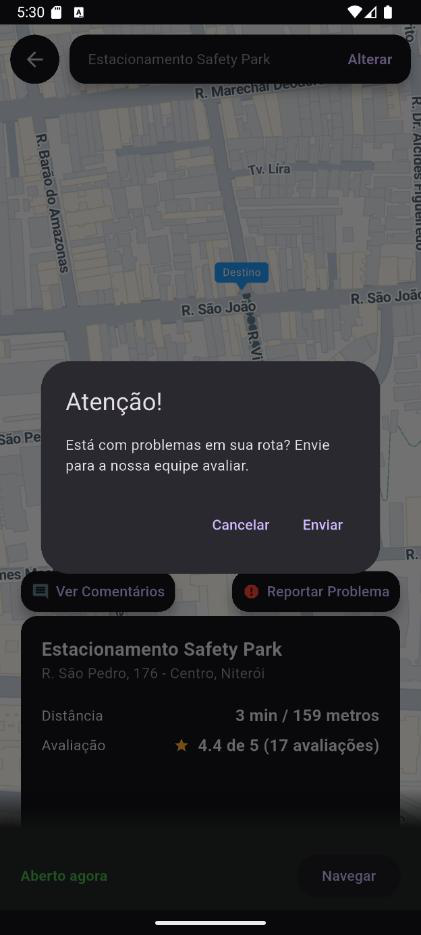
\includegraphics[height=0.34\textheight,keepaspectratio]{capitulos/figuras/emulador-reportar.png}
      \caption{Aplicação rodando no emulador – Reportar problemas}
      \label{fig:emulador-reportar}
   \end{minipage}\hfill
   \begin{minipage}[b]{0.48\linewidth}
      \centering
      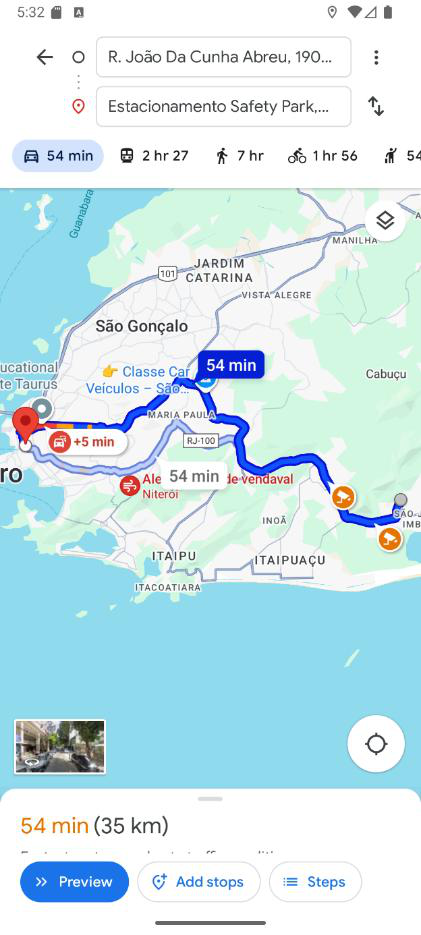
\includegraphics[height=0.34\textheight,keepaspectratio]{capitulos/figuras/emulador-navegacao.png}
      \caption{Aplicação rodando no emulador - Tela de navegação do google maps}
      \label{fig:emulador-navegacao}
   \end{minipage}
\end{figure}

A \autoref{fig:emulador-reportar} apresenta a tela de reportar problemas do aplicativo Parkon, permitindo ao usuário informar à equipe sobre dificuldades encontradas na rota até o estacionamento. A \autoref{fig:emulador-navegacao} mostra a tela de navegação do Google Maps integrada ao aplicativo, exibindo o trajeto detalhado até o estacionamento selecionado.

\begin{figure}[H]
   \centering
   \begin{minipage}[b]{0.48\linewidth}
      \centering
      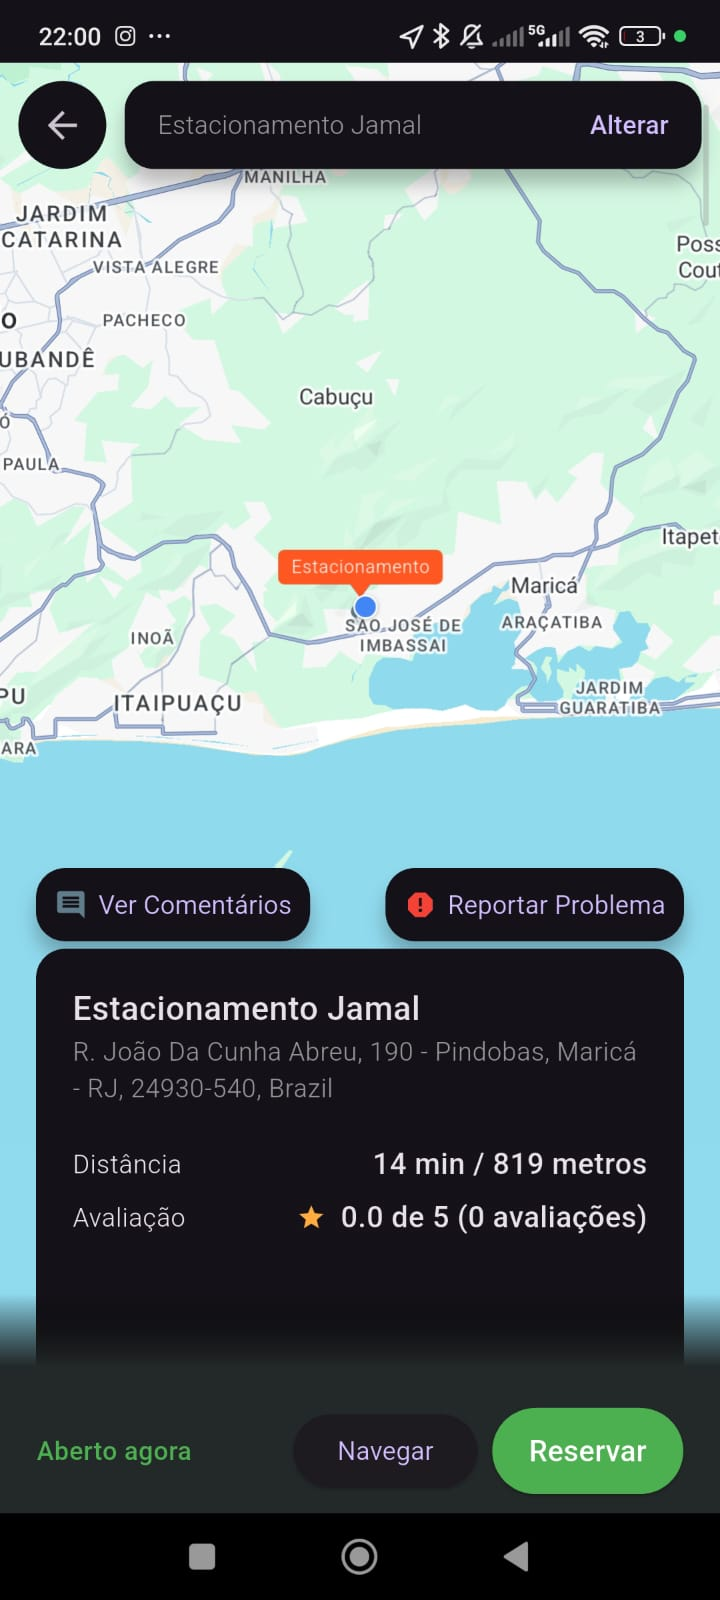
\includegraphics[height=0.34\textheight,keepaspectratio]{capitulos/figuras/app-reservar.jpeg}
      \caption{Aplicação rodando no emulador - Detalhes do estacionamento credenciado}
      \label{fig:app-reservar}
   \end{minipage}\hfill
   \begin{minipage}[b]{0.48\linewidth}
      \centering
      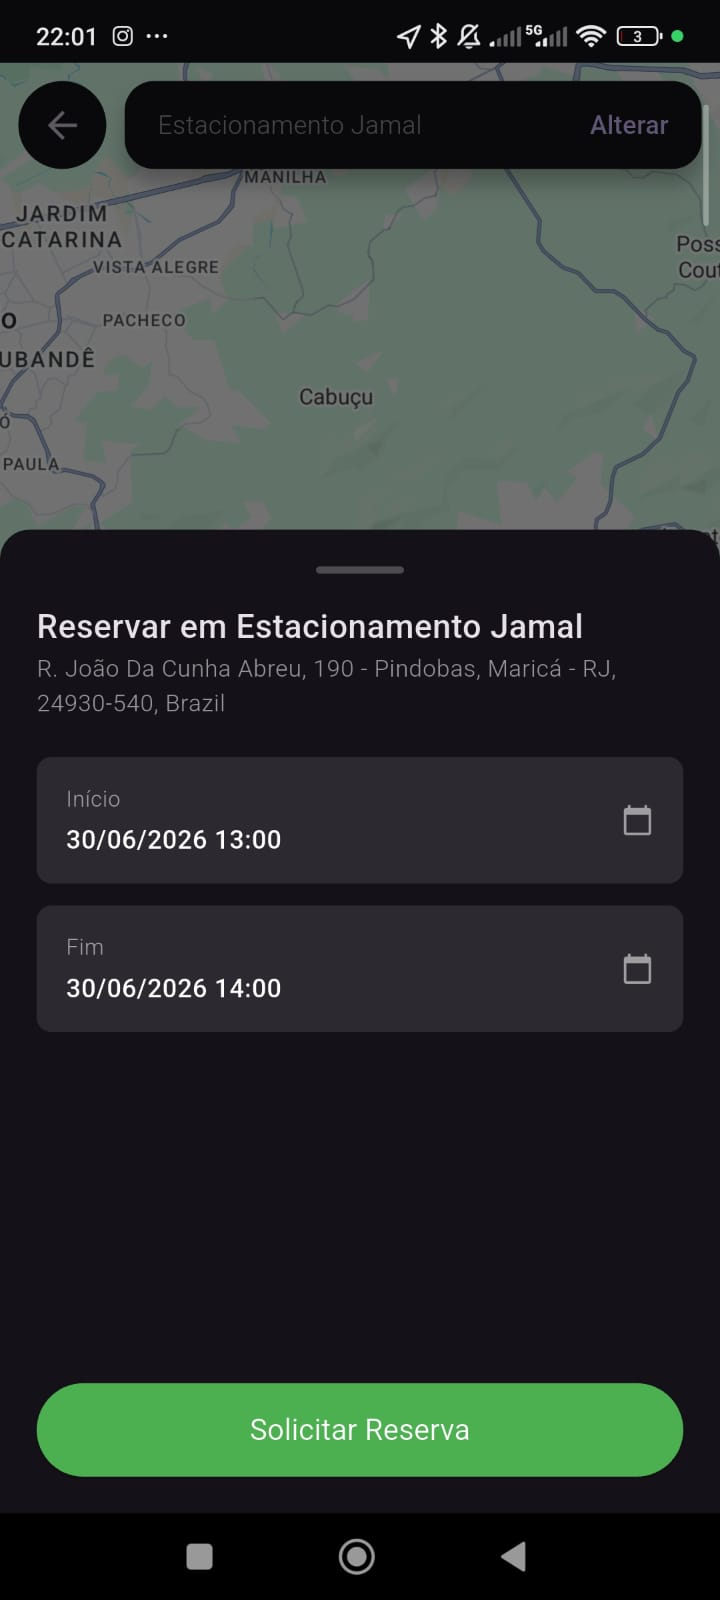
\includegraphics[height=0.34\textheight,keepaspectratio]{capitulos/figuras/app-reservar-data.jpeg}
      \caption{Aplicação rodando no emulador - Seleção de data e hora da reserva}
      \label{fig:app-reservar-data}
   \end{minipage}
\end{figure}

\begin{figure}[H]
   \centering
   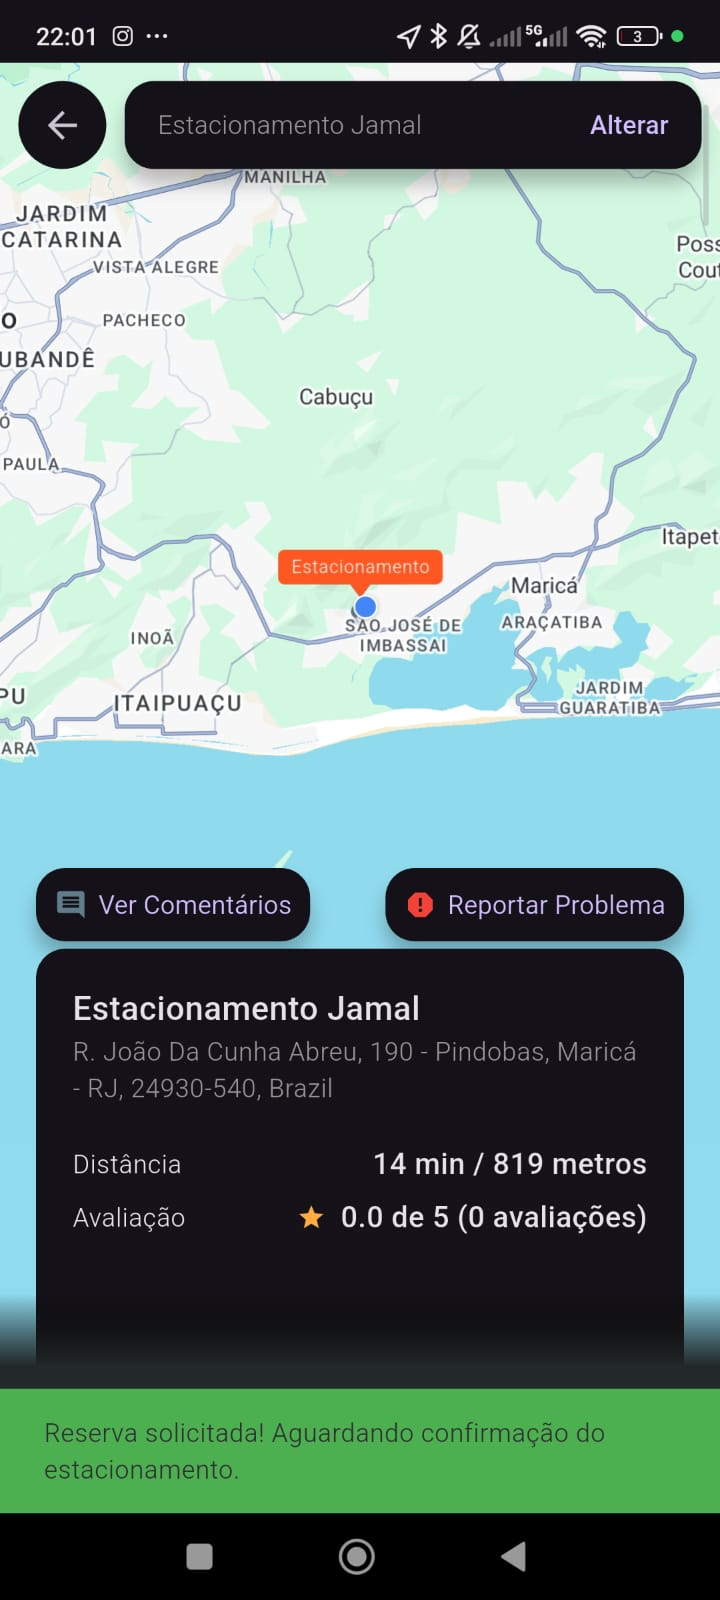
\includegraphics[height=0.34\textheight,keepaspectratio]{capitulos/figuras/app-reservado.jpeg}
   \caption{Aplicação rodando no emulador - Reserva solicitada aguardando confirmação}
   \label{fig:app-reservado}
\end{figure}

A \autoref{fig:app-reservar} apresenta a tela de detalhes de um estacionamento credenciado na plataforma, exibindo a localização no mapa, endereço, distância, avaliação e os botões de ação ``Ver Comentários'', ``Reportar Problema'', ``Navegar'' e ``Reservar''. A \autoref{fig:app-reservar-data} mostra a tela de reserva, onde o usuário seleciona a data e hora de início e fim da reserva e confirma com o botão ``Solicitar Reserva''. A \autoref{fig:app-reservado} apresenta a confirmação da solicitação, com o banner informando que a reserva foi solicitada e aguarda confirmação do administrador do estacionamento.

\subsection{Telas do Portal Web}
\label{sec:telas-web}

\begin{figure}[H]
   \centering
   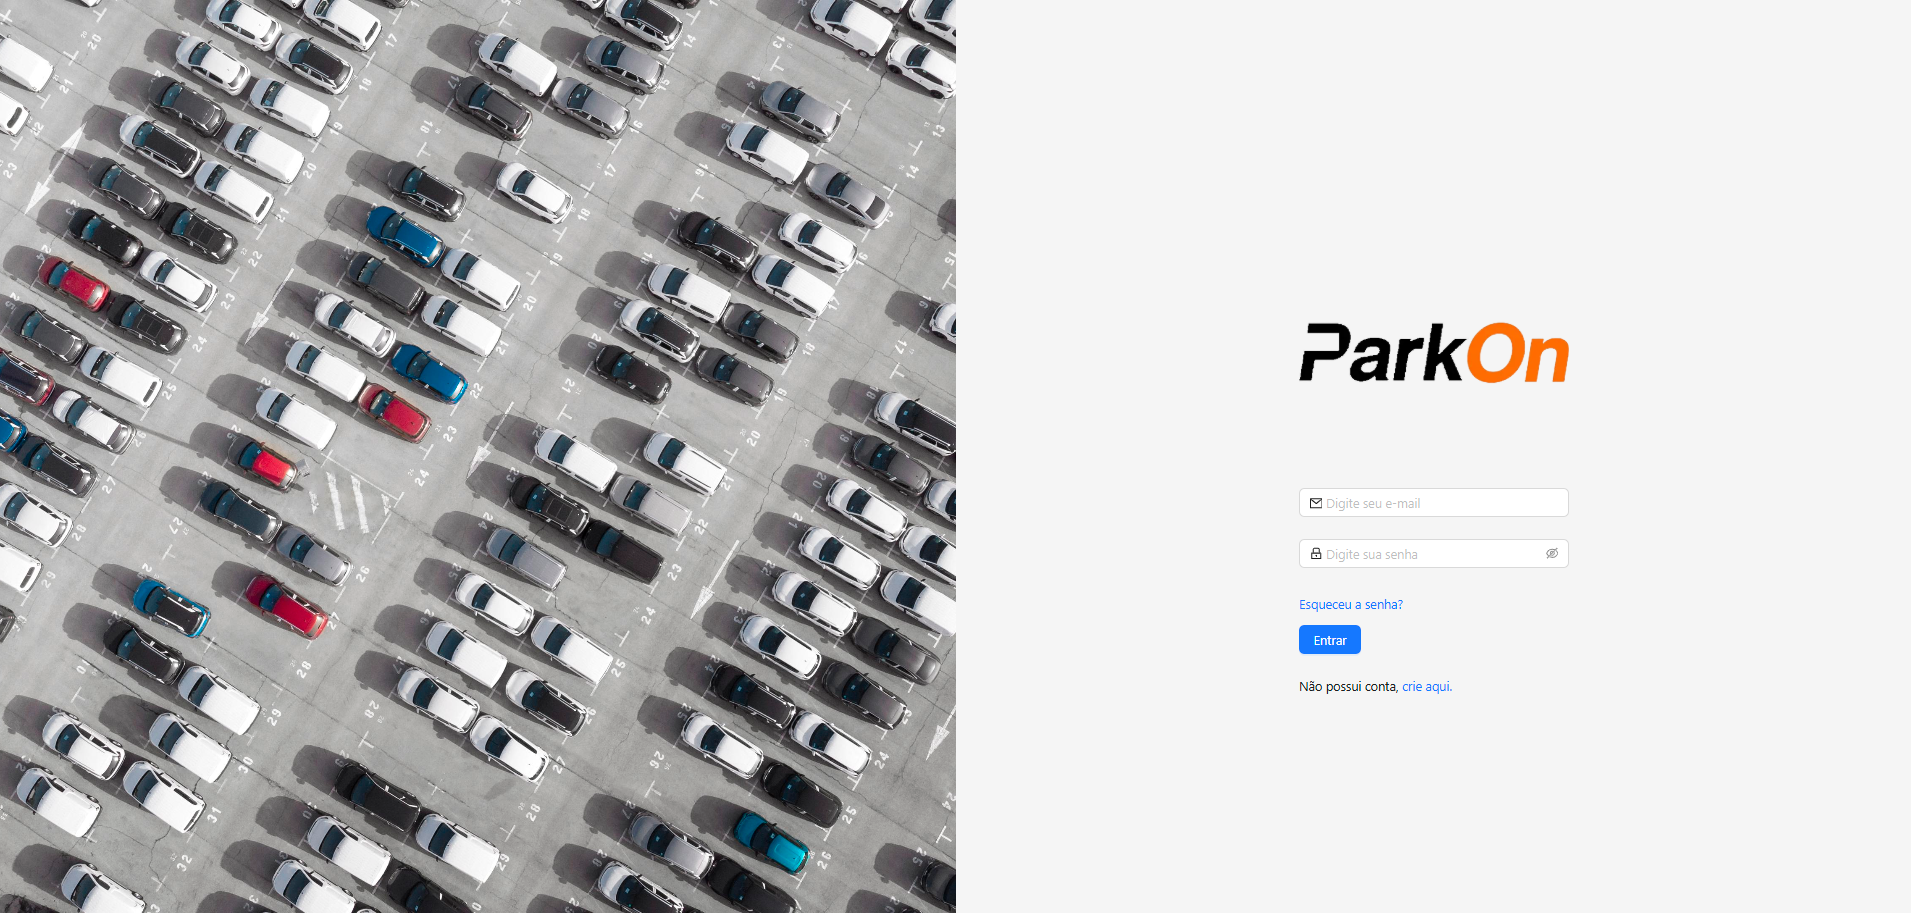
\includegraphics[width=0.85\linewidth]{capitulos/figuras/portal-login.png}
   \caption{Portal Web - Tela de Login}
   \label{fig:portal-login}
\end{figure}

\begin{figure}[H]
   \centering
   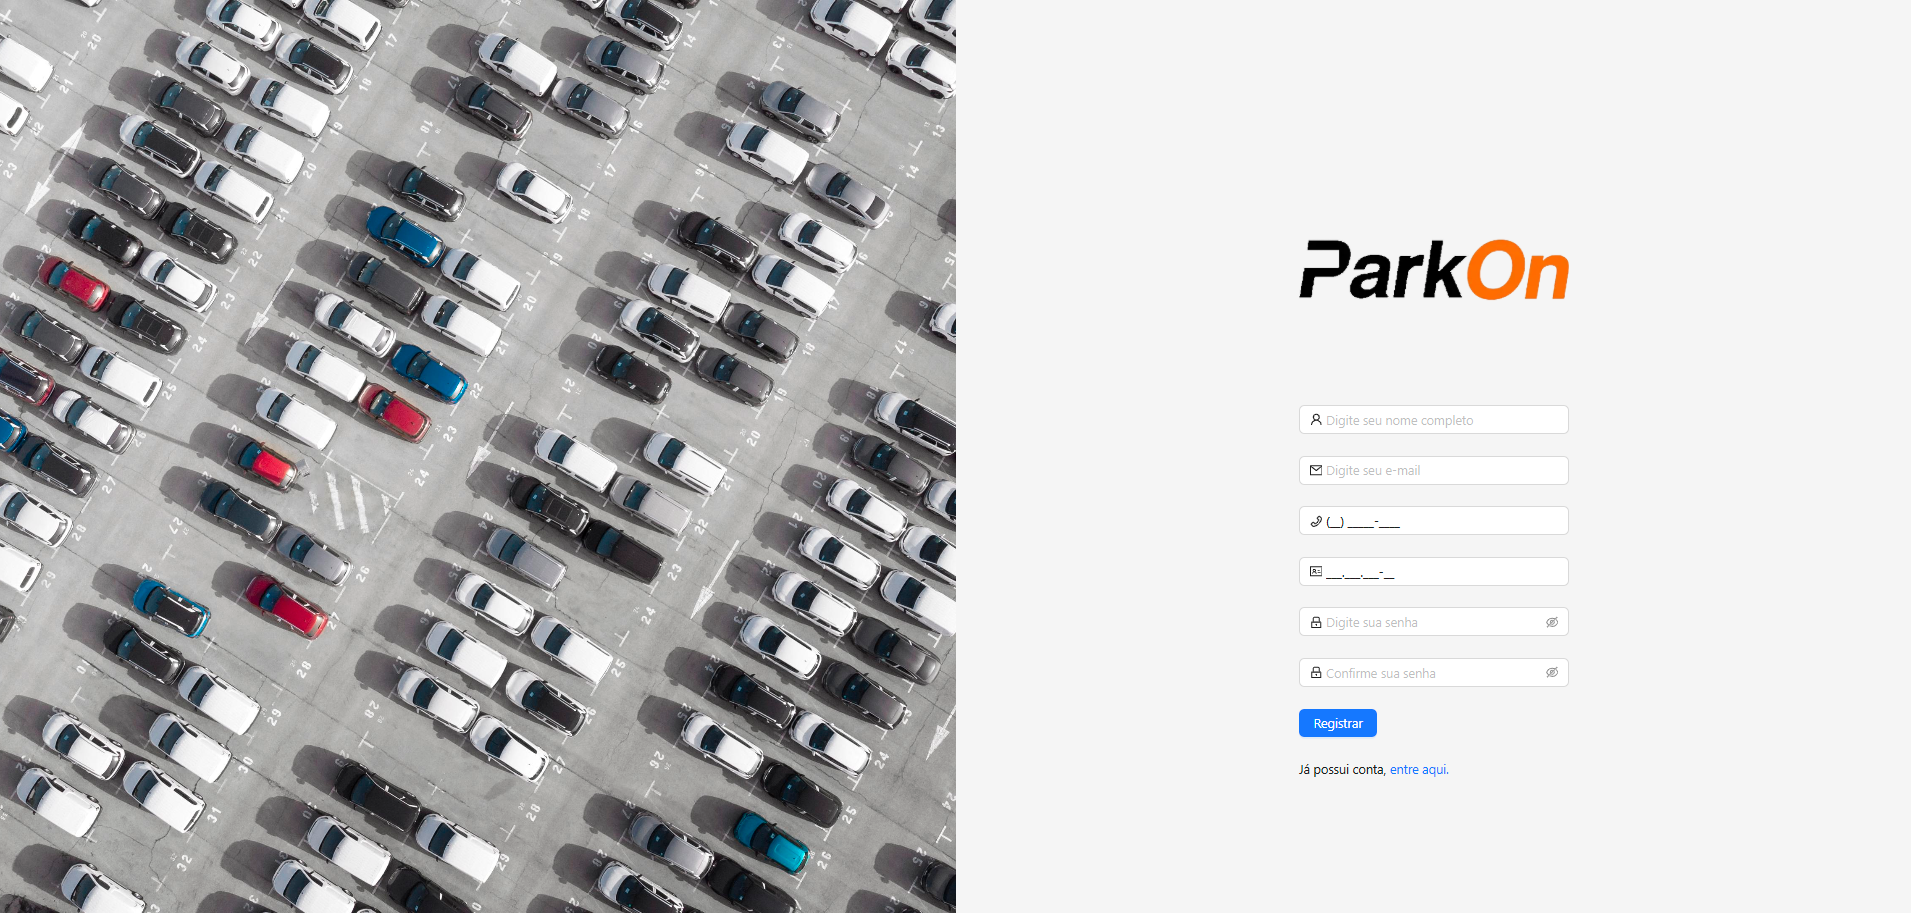
\includegraphics[width=0.85\linewidth]{capitulos/figuras/portal-cadastro.png}
   \caption{Portal Web - Tela de Cadastro}
   \label{fig:portal-cadastro}
\end{figure}

A \autoref{fig:portal-login} apresenta a tela de login do portal web administrativo ParkOn, onde o administrador do estacionamento pode inserir e-mail e senha para acessar o painel de gestão. Já a \autoref{fig:portal-cadastro} mostra a tela de cadastro, onde o administrador informa nome completo, e-mail, telefone, CPF, senha e confirmação de senha para criar sua conta na plataforma.

\begin{figure}[H]
   \centering
   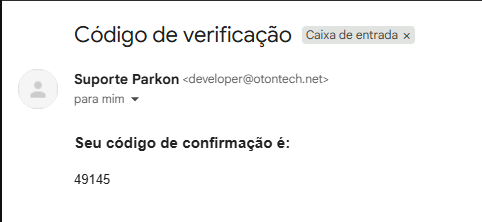
\includegraphics[width=0.85\linewidth]{capitulos/figuras/portal-confirmacao-email.png}
   \caption{Portal Web - E-mail com código de verificação}
   \label{fig:portal-confirmacao-email}
\end{figure}

\begin{figure}[H]
   \centering
   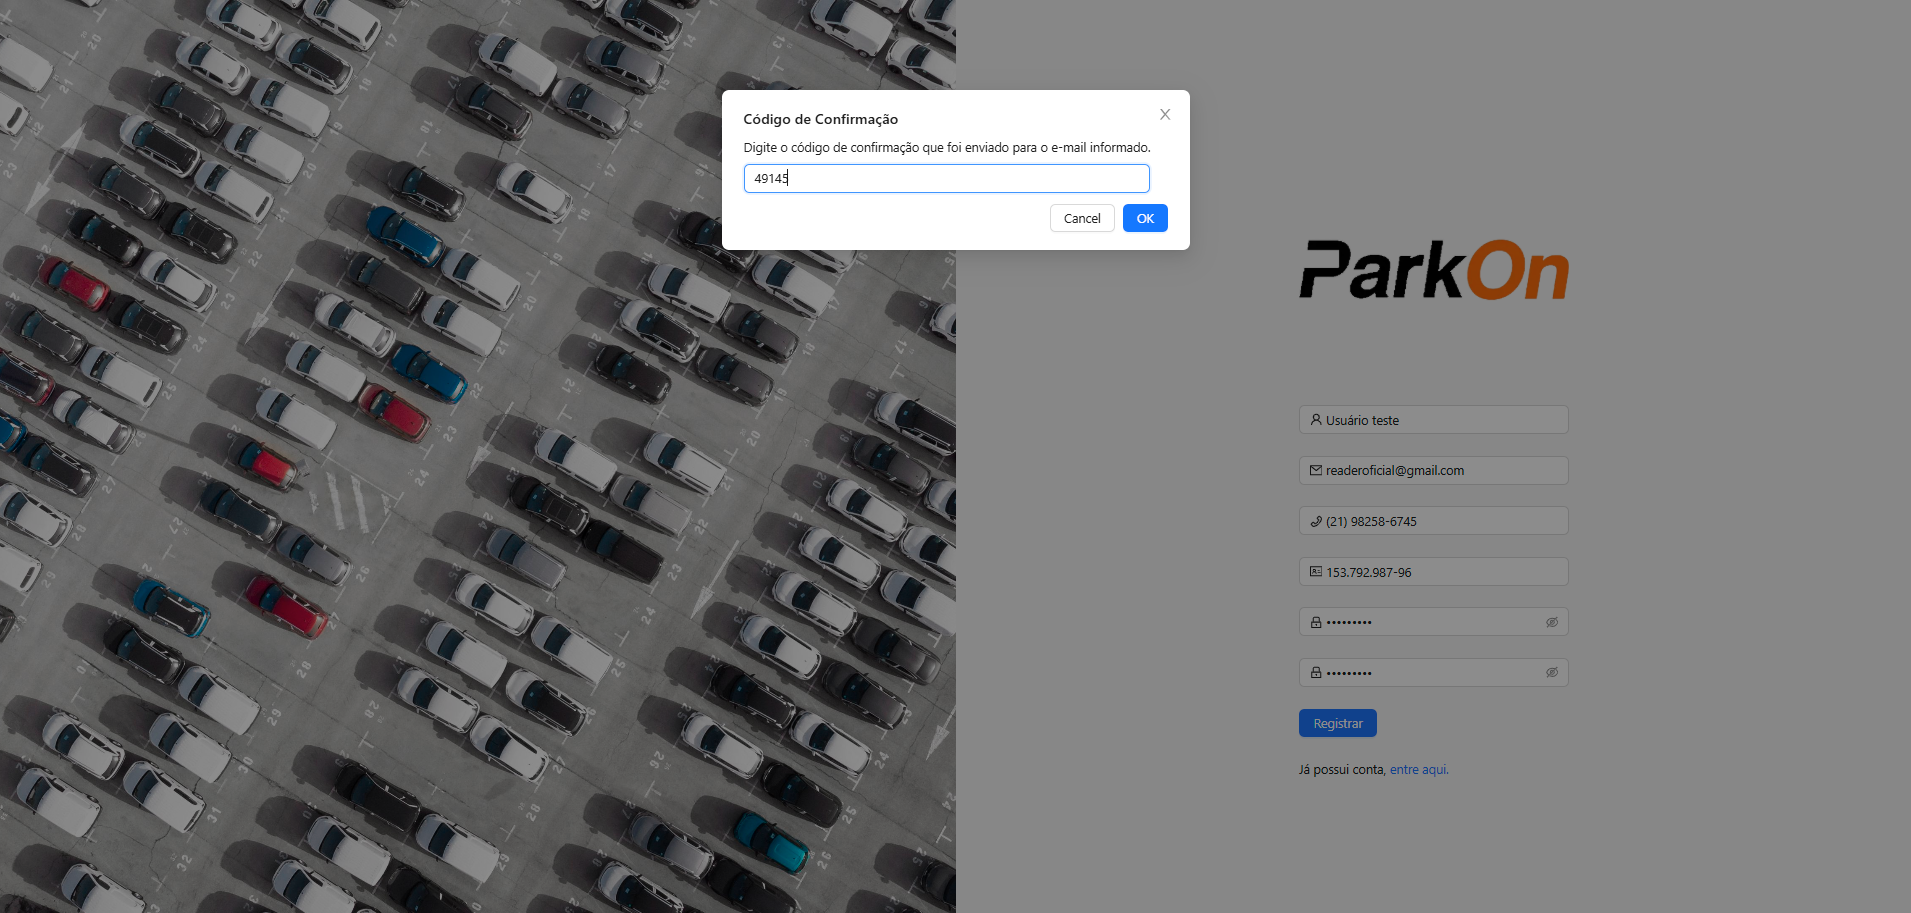
\includegraphics[width=0.85\linewidth]{capitulos/figuras/portal-confirmacao.png}
   \caption{Portal Web - Modal de confirmação de código}
   \label{fig:portal-confirmacao}
\end{figure}

A \autoref{fig:portal-confirmacao-email} mostra o e-mail enviado ao administrador com o código de verificação necessário para concluir o cadastro na plataforma. A \autoref{fig:portal-confirmacao} apresenta o modal de confirmação exibido sobre a tela de cadastro, onde o administrador insere o código recebido por e-mail para validar sua conta.

\begin{figure}[H]
   \centering
   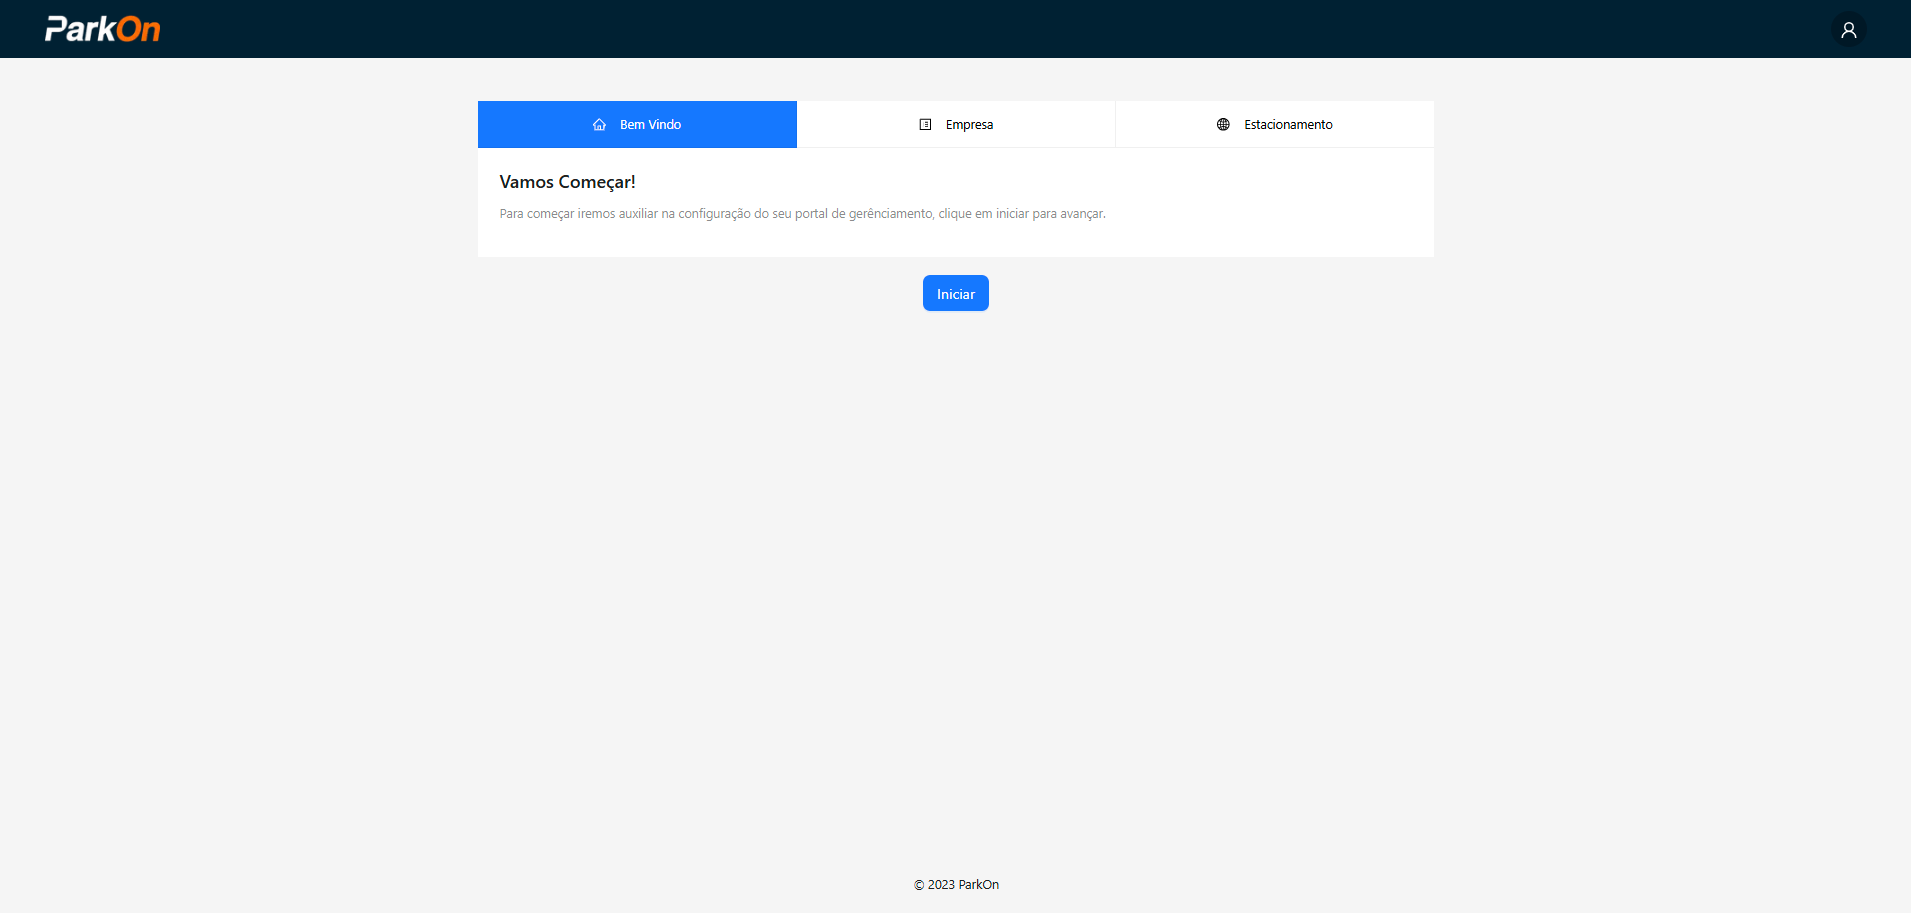
\includegraphics[width=0.85\linewidth]{capitulos/figuras/portal-setup-1.png}
   \caption{Portal Web - Configuração inicial (Bem Vindo)}
   \label{fig:portal-setup-1}
\end{figure}

\begin{figure}[H]
   \centering
   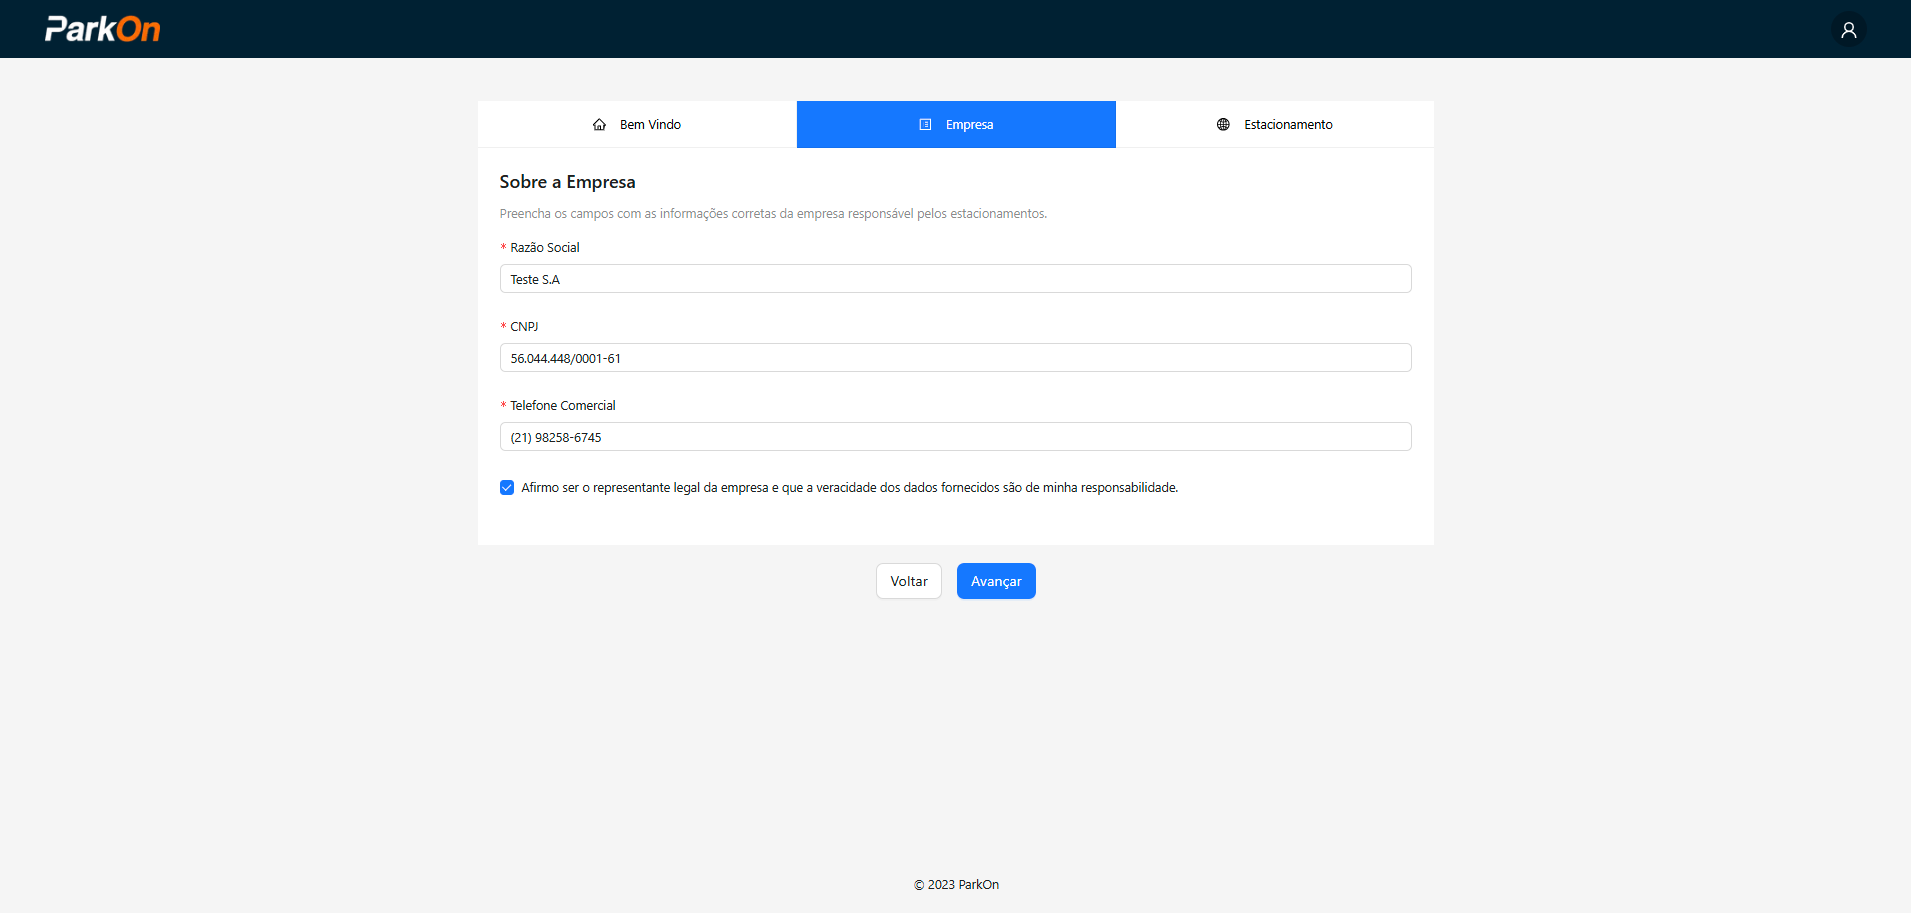
\includegraphics[width=0.85\linewidth]{capitulos/figuras/portal-setup-2.png}
   \caption{Portal Web - Configuração inicial (Dados da Empresa)}
   \label{fig:portal-setup-2}
\end{figure}

\begin{figure}[H]
   \centering
   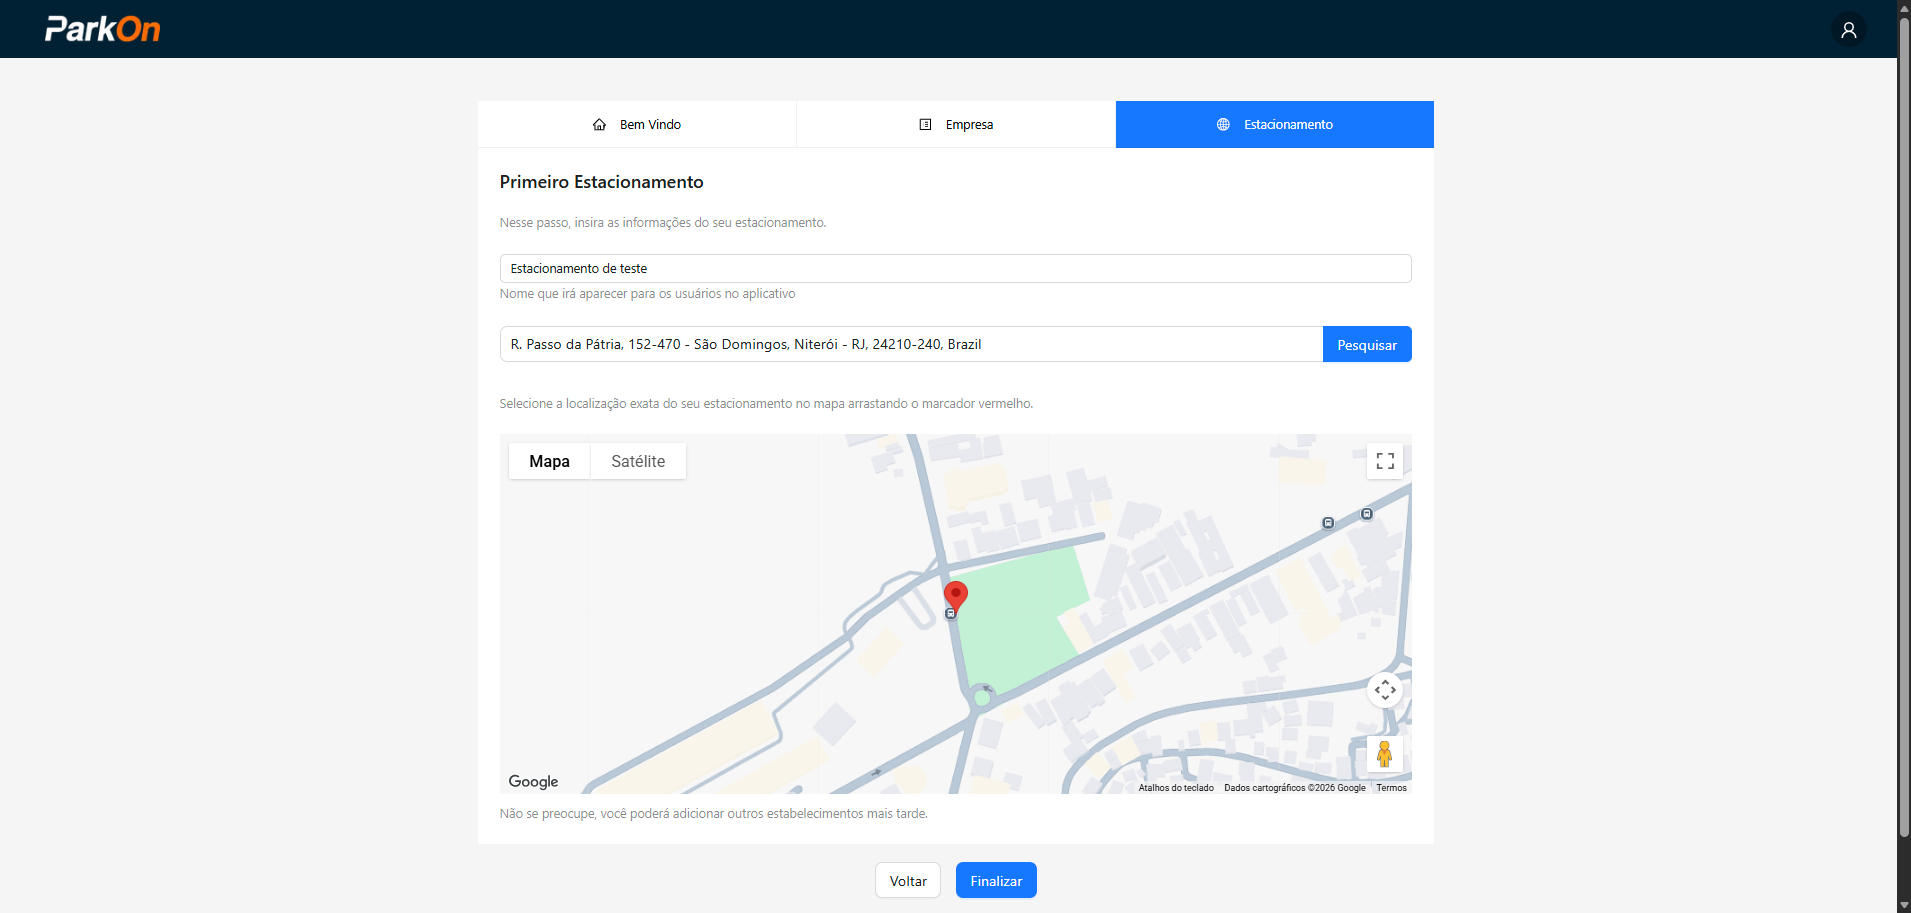
\includegraphics[width=0.85\linewidth]{capitulos/figuras/portal-setup-3.png}
   \caption{Portal Web - Configuração inicial (Primeiro Estacionamento)}
   \label{fig:portal-setup-3}
\end{figure}

Após a validação do cadastro, o administrador é direcionado para o assistente de configuração inicial. A \autoref{fig:portal-setup-1} apresenta a tela de boas-vindas com o botão ``Iniciar''. A \autoref{fig:portal-setup-2} mostra o formulário de cadastro da empresa, com campos para razão social, CNPJ e telefone comercial, além de uma declaração de responsabilidade sobre os dados informados. A \autoref{fig:portal-setup-3} apresenta o cadastro do primeiro estacionamento, onde o administrador informa o nome do estabelecimento e o endereço, com integração ao Google Maps para posicionamento no mapa.

\begin{figure}[H]
   \centering
   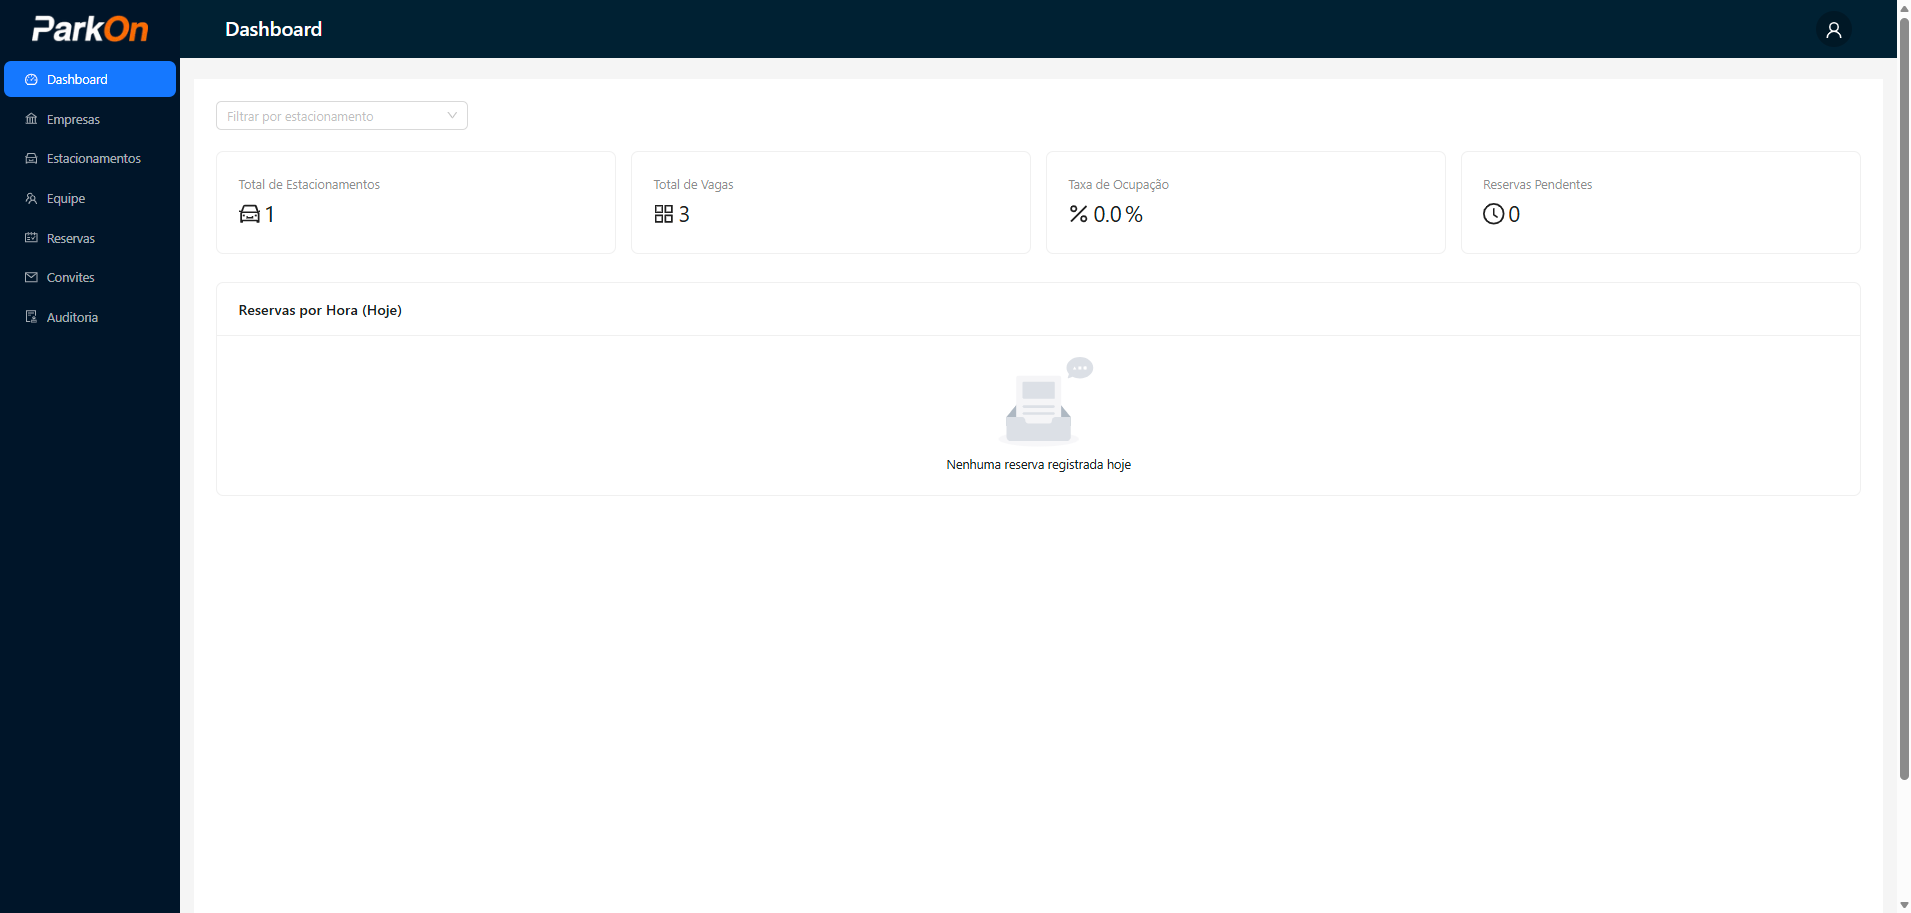
\includegraphics[width=0.85\linewidth]{capitulos/figuras/portal-dashboard.png}
   \caption{Portal Web - Dashboard}
   \label{fig:portal-dashboard}
\end{figure}

A \autoref{fig:portal-dashboard} apresenta o painel principal do portal administrativo, exibindo métricas como total de estacionamentos, total de vagas, taxa de ocupação e reservas pendentes, além de um gráfico de reservas por hora. O menu lateral permite acesso rápido às demais funcionalidades do sistema.

\begin{figure}[H]
   \centering
   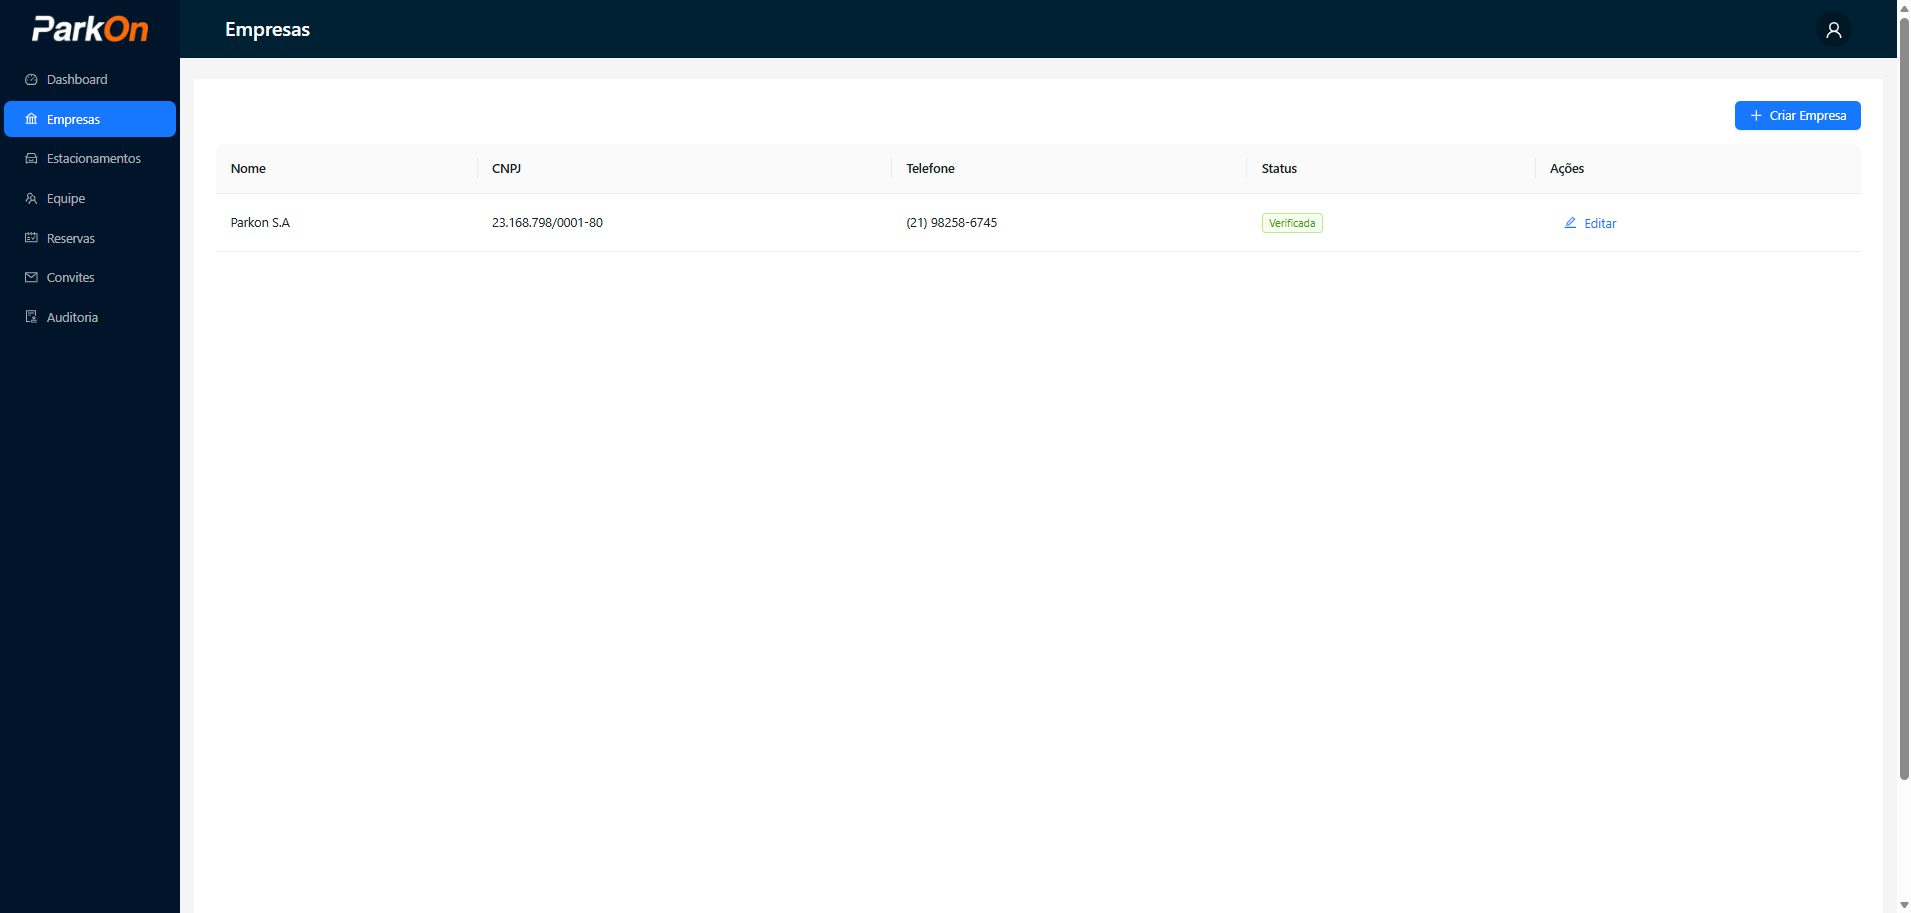
\includegraphics[width=0.85\linewidth]{capitulos/figuras/portal-empresas.png}
   \caption{Portal Web - Gerenciamento de Empresas}
   \label{fig:portal-empresas}
\end{figure}

A \autoref{fig:portal-empresas} mostra a tela de gerenciamento de empresas, onde o administrador pode visualizar as empresas cadastradas com informações como nome, CNPJ, telefone, status de verificação e ações disponíveis, além de criar novas empresas.

\begin{figure}[H]
   \centering
   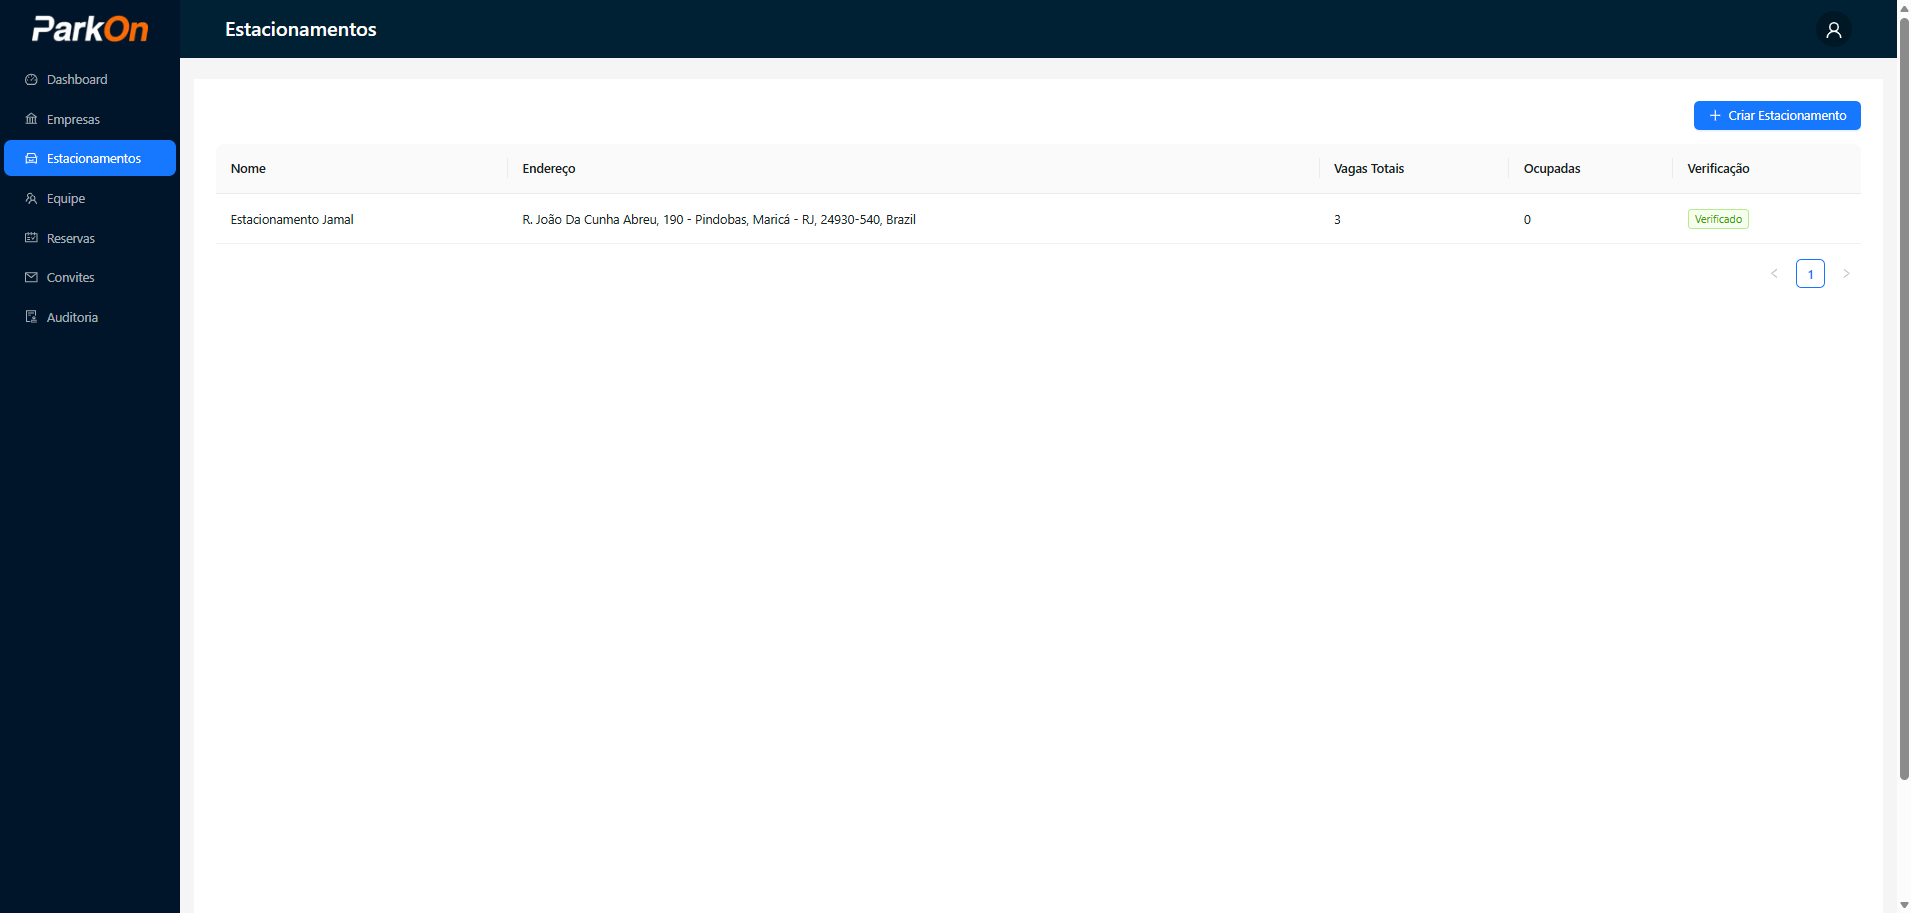
\includegraphics[width=0.85\linewidth]{capitulos/figuras/portal-estacionamentos.png}
   \caption{Portal Web - Lista de Estacionamentos}
   \label{fig:portal-estacionamentos}
\end{figure}

A \autoref{fig:portal-estacionamentos} apresenta a lista de estacionamentos cadastrados, exibindo nome, endereço, vagas totais, vagas ocupadas e status de verificação, com a opção de criar novos estacionamentos.

\begin{figure}[H]
   \centering
   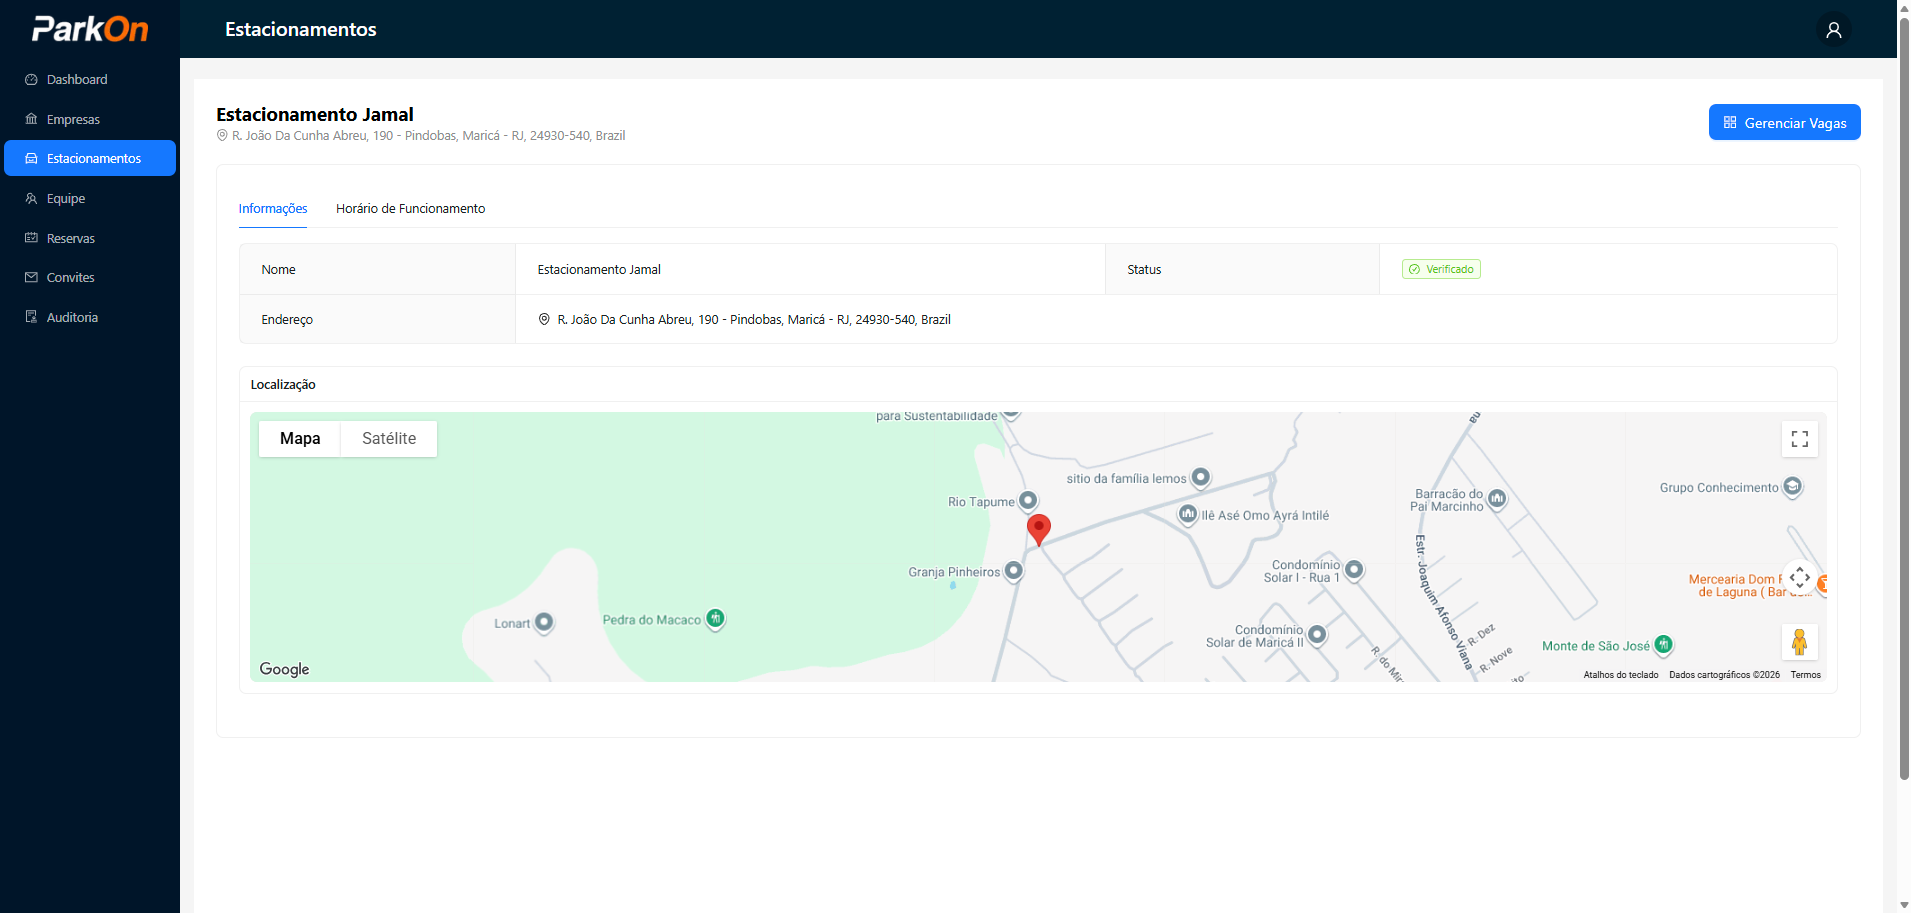
\includegraphics[width=0.85\linewidth]{capitulos/figuras/portal-edicao-estacionamento.png}
   \caption{Portal Web - Detalhes do Estacionamento (Informações)}
   \label{fig:portal-edicao-estacionamento}
\end{figure}

\begin{figure}[H]
   \centering
   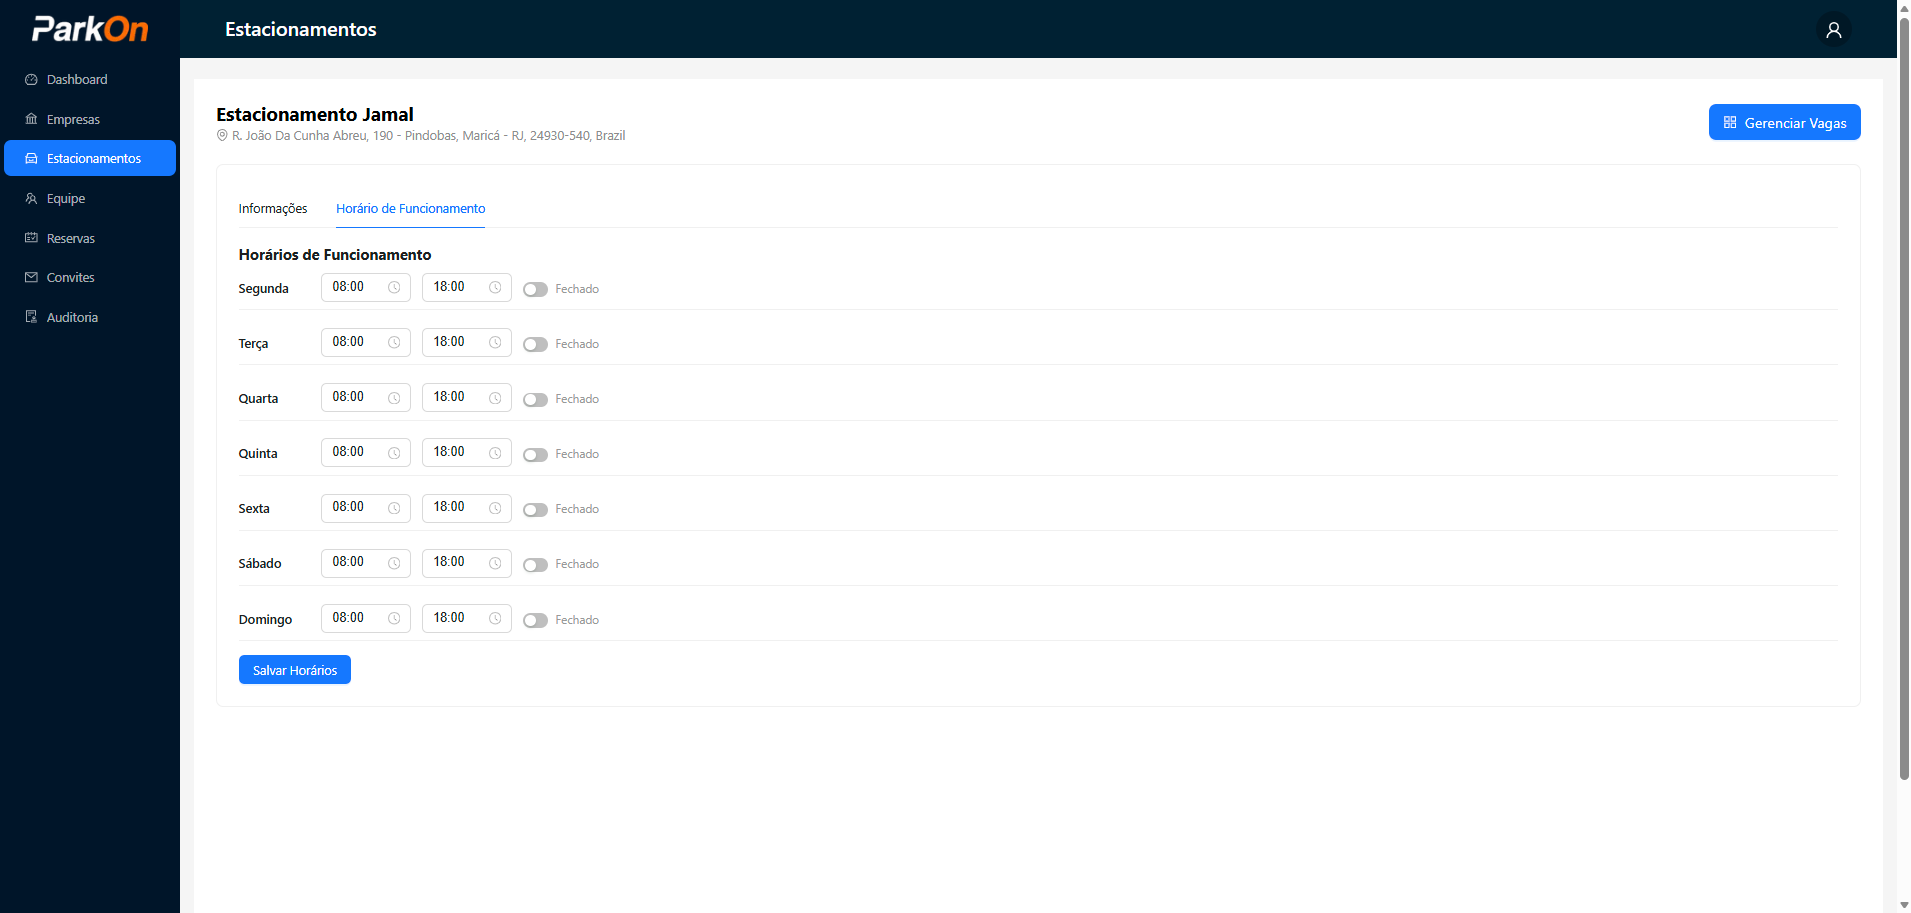
\includegraphics[width=0.85\linewidth]{capitulos/figuras/portal-edicao-estacionamento-horario.png}
   \caption{Portal Web - Detalhes do Estacionamento (Horários de Funcionamento)}
   \label{fig:portal-edicao-estacionamento-horario}
\end{figure}

A \autoref{fig:portal-edicao-estacionamento} mostra a tela de detalhes do estacionamento com informações gerais (nome, endereço, status) e a localização no mapa. A \autoref{fig:portal-edicao-estacionamento-horario} apresenta a configuração dos horários de funcionamento por dia da semana, com opção de marcar dias como fechado.

\begin{figure}[H]
   \centering
   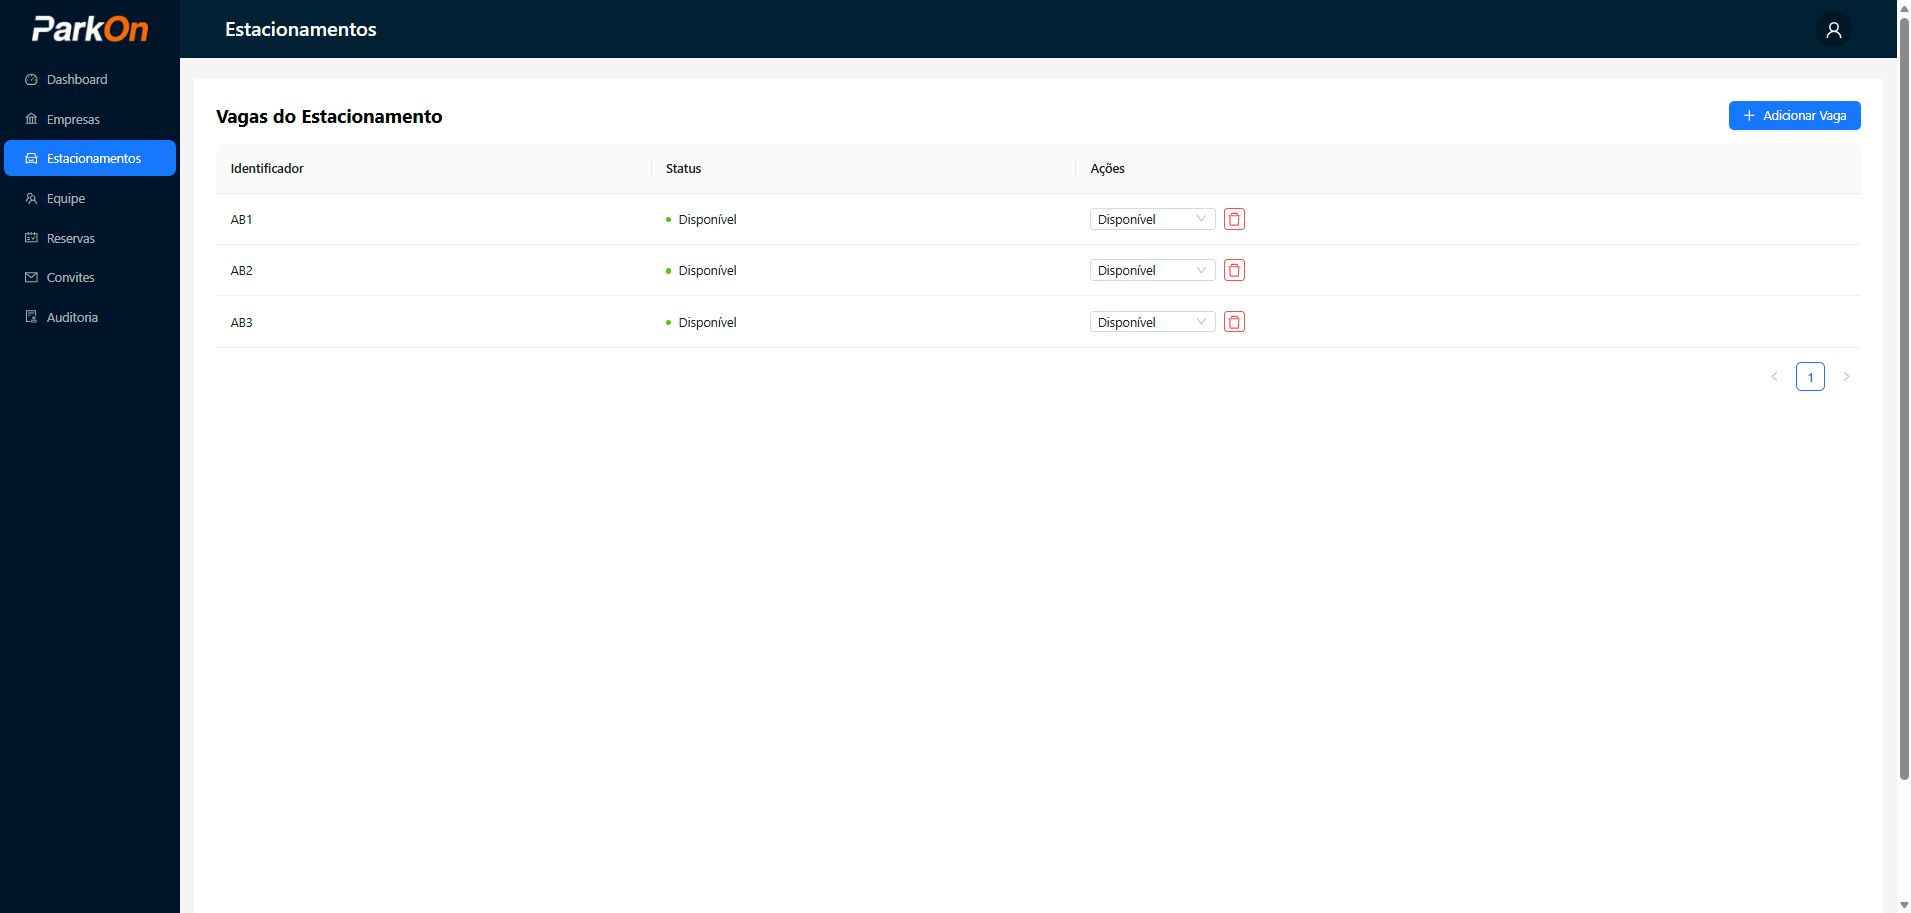
\includegraphics[width=0.85\linewidth]{capitulos/figuras/portal-edicao-estacionamento-vagas.png}
   \caption{Portal Web - Gerenciamento de Vagas}
   \label{fig:portal-edicao-estacionamento-vagas}
\end{figure}

A \autoref{fig:portal-edicao-estacionamento-vagas} apresenta a tela de gerenciamento de vagas do estacionamento, onde o administrador pode visualizar o identificador e o status de cada vaga, alterar sua disponibilidade e adicionar novas vagas.

\begin{figure}[H]
   \centering
   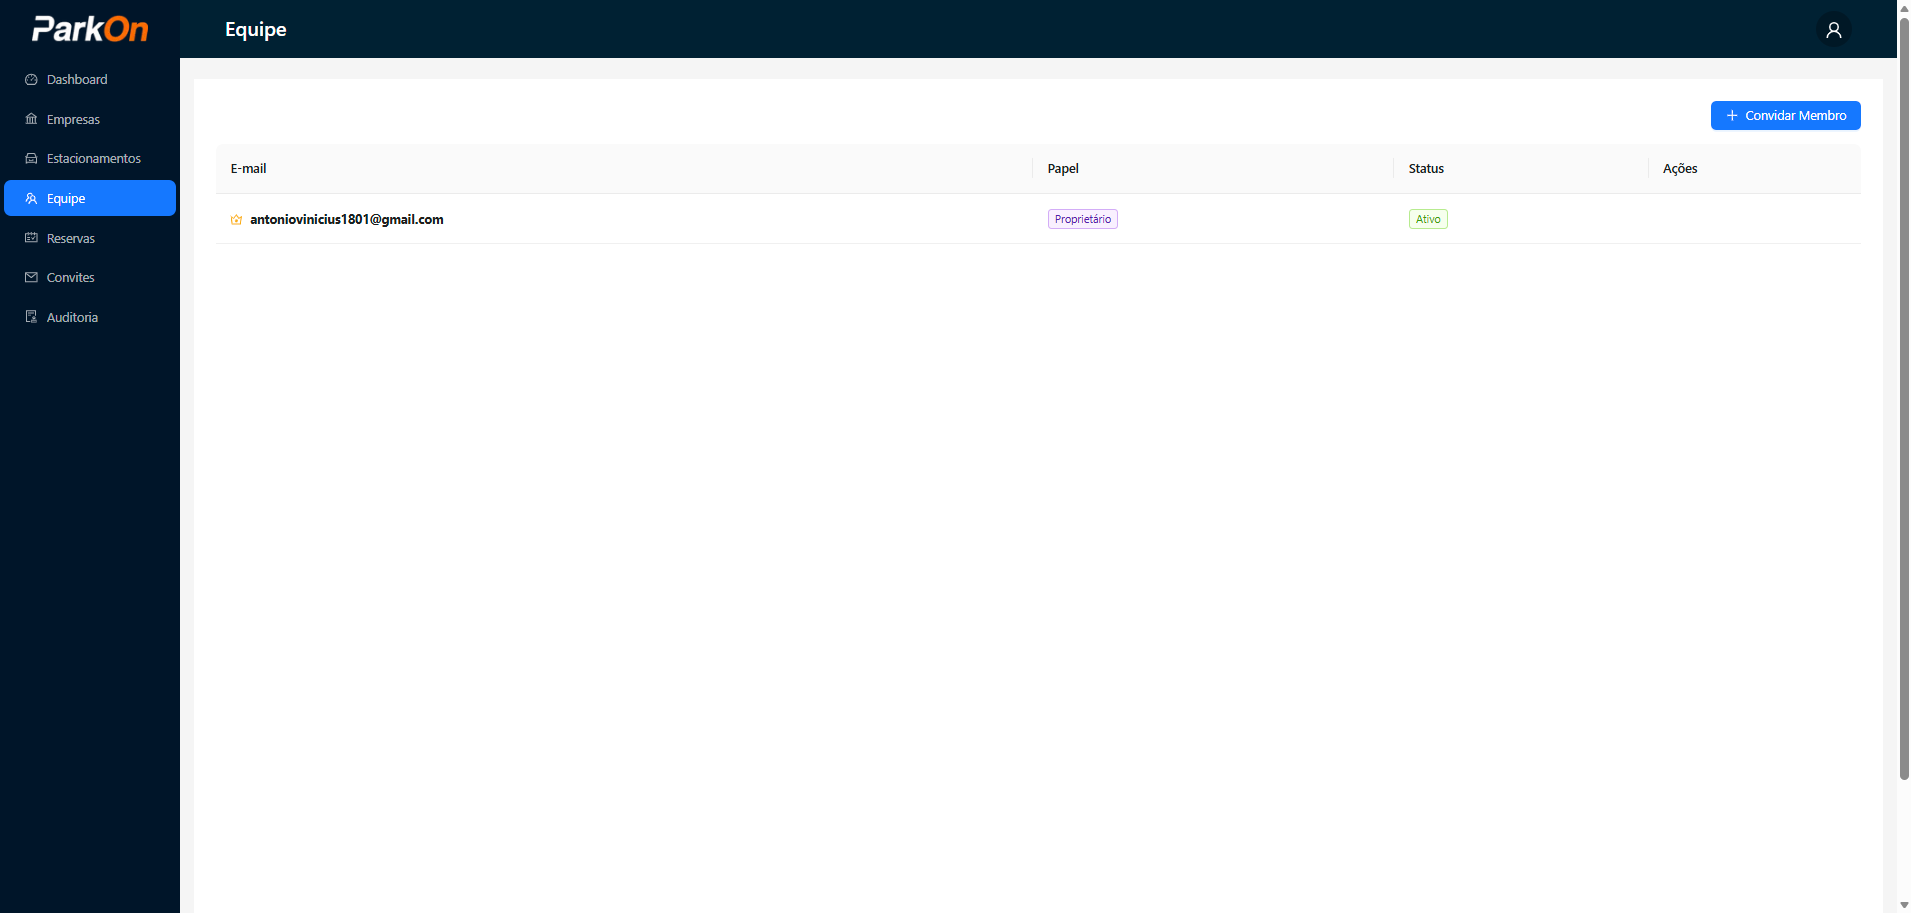
\includegraphics[width=0.85\linewidth]{capitulos/figuras/portal-equipe.png}
   \caption{Portal Web - Gerenciamento de Equipe}
   \label{fig:portal-equipe}
\end{figure}

A \autoref{fig:portal-equipe} mostra a tela de gerenciamento de equipe, onde o administrador visualiza os membros com seus respectivos papéis e status, além de poder convidar novos colaboradores para auxiliar na gestão do estacionamento.

\begin{figure}[H]
   \centering
   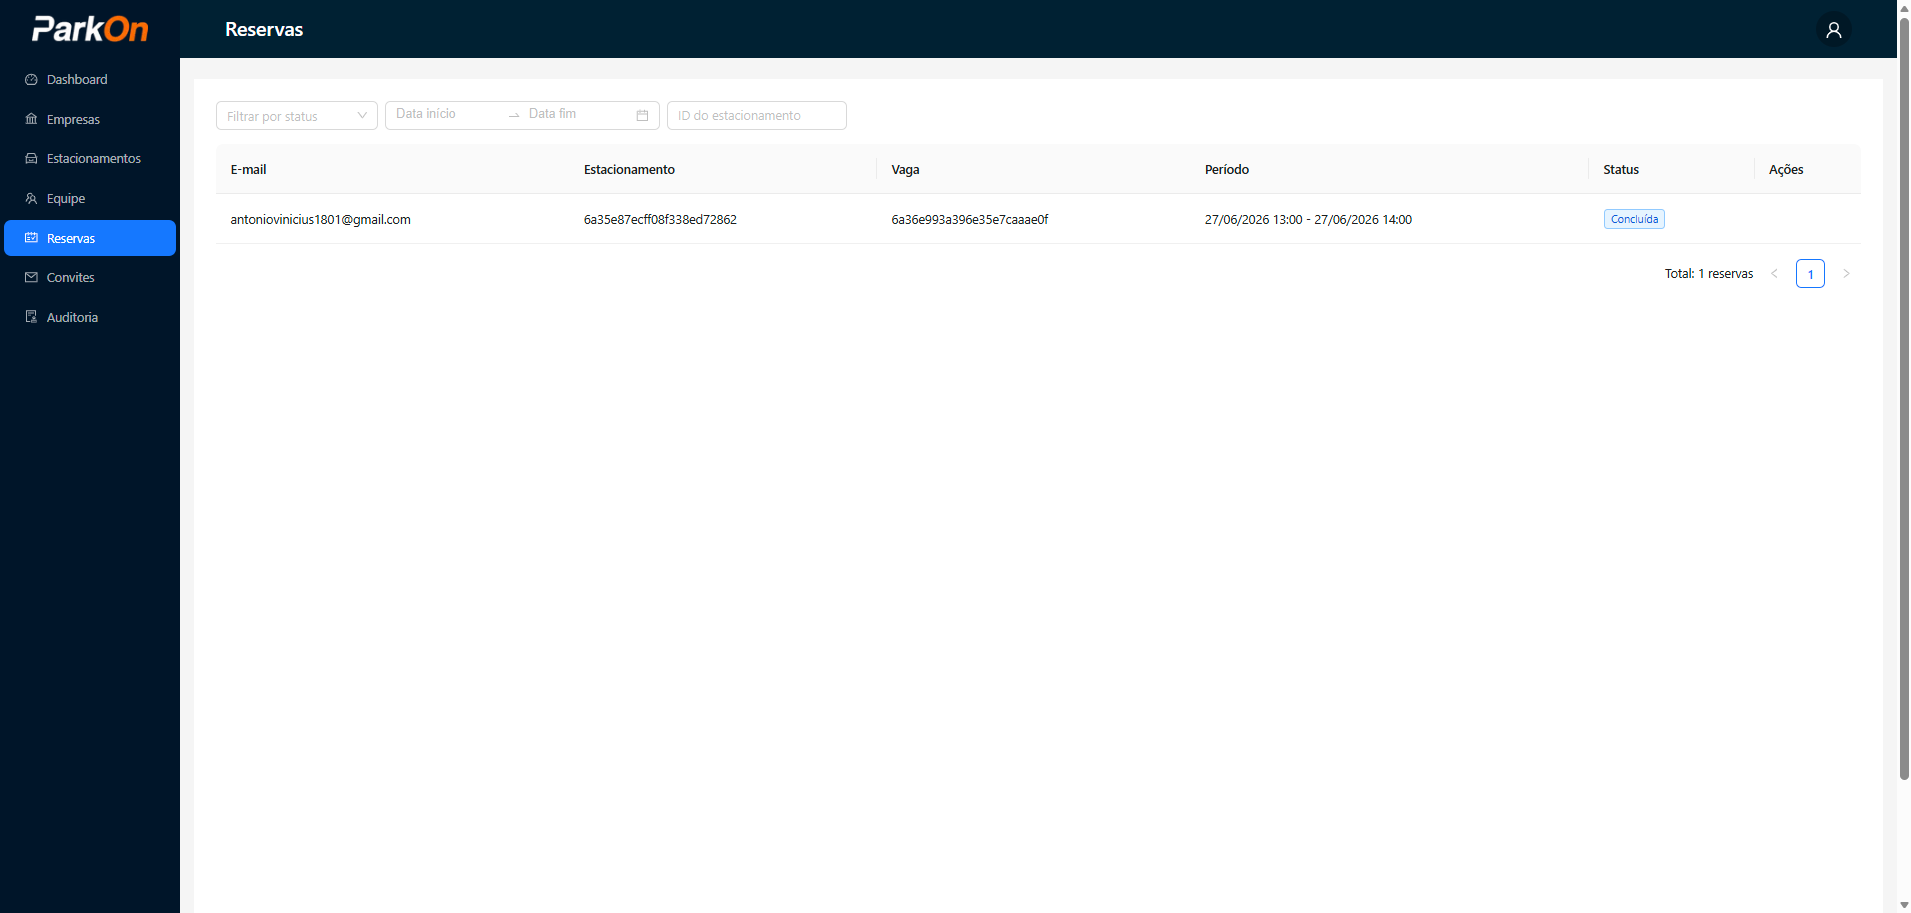
\includegraphics[width=0.85\linewidth]{capitulos/figuras/portal-reservas.png}
   \caption{Portal Web - Gerenciamento de Reservas}
   \label{fig:portal-reservas}
\end{figure}

A \autoref{fig:portal-reservas} apresenta a tela de gerenciamento de reservas, exibindo informações como e-mail do usuário, estacionamento, vaga, período, status e ações disponíveis, permitindo ao administrador acompanhar e gerenciar as reservas realizadas pelos motoristas.

\section{Build do Aplicativo}
\label{sec:build-aplicativo}

O processo de build da plataforma Parkon envolve três componentes distintos: o aplicativo mobile (Flutter), o backend (Go) e o portal web administrativo (Next.js). Para cada um, foram utilizados comandos \acrfull{cli} que automatizam a criação dos artefatos para distribuição e execução.

\subsection{Build do Aplicativo Mobile (Flutter)}
\label{sec:build-mobile}

O aplicativo mobile foi desenvolvido utilizando o framework Flutter~\cite{gradin2025}, que permite a geração de pacotes para múltiplas plataformas, como Android e iOS, a partir de uma única base de código. Exemplos de comandos utilizados:

\begin{verbatim}
# Build para Android (APK)
flutter build apk --release

# Build para Android (App Bundle)
flutter build appbundle --release

# Build para iOS (necessário macOS)
flutter build ios --release
\end{verbatim}

Esses comandos geram os pacotes necessários para publicação nas lojas de aplicativos ou para testes em dispositivos físicos.

\subsection{Build do Backend (Go)}
\label{sec:build-backend}

O backend do sistema foi desenvolvido em Go, proporcionando alta performance e facilidade de escalabilidade. O processo de build do backend é realizado via linha de comando:

\begin{verbatim}
# Compilar o backend
go build -o parkon-backend main.go

# Executar o backend localmente
./parkon-backend

# Para rodar em ambiente de produção com Docker:
docker build -t parkon-backend .
docker run -d -p 8080:8080 parkon-backend
\end{verbatim}

Esses comandos garantem que o backend esteja pronto para execução local ou implantação em ambientes cloud, facilitando a integração com o aplicativo mobile e o portal web.

\subsection{Build do Portal Web (Next.js)}
\label{sec:build-portal-web}

O processo de build do portal web é realizado via linha de comando:

\begin{verbatim}
# Instalar dependências
npm install

# Executar em ambiente de desenvolvimento
npm run dev

# Build para produção
npm run build

# Iniciar em produção
npm start
\end{verbatim}

% ---------------------------------------------------------------------
% --- CAPÍTULO 5 - CONCLUSÕES
% --- Conteúdo extraído VERBATIM de TCC_PARKON_V3.pdf (página 31),
% --- fonte da verdade. Fragmento LaTeX (sem \documentclass/preâmbulo),
% --- incluído via \include em tese.tex. Arquivo em UTF-8.
% ---
% --- Título de origem (corpo do PDF): "CONCLUSÕES" (capítulo 5).
% ---   A classe PPGC_UFF formata o título do capítulo em maiúsculas;
% ---   por isso usa-se \chapter{Conclusões} (mesma saída visível),
% ---   mantendo a coerência com cap1.tex/cap2.tex (Requisitos 1.2 e 1.6).
% ---   \label{cap:conclusao} preservado conforme convenção do projeto
% ---   (referenciado por \autoref em cap1.tex).
% ---
% --- MAPEAMENTO DE CITAÇÕES (fonte usa numeração [n]; convertidas para \cite):
% ---   [2]  -> \cite{flutter2025}    "Application development using flutter" (sem autor; @misc/online)
% ---   [10] -> \cite{goldstein2025}  GOLDSTEIN, S. "Criação de plataforma de geocoding baseada em serviços Google Maps"
% ---   TODO: [CITATION] As referências da fonte NÃO trazem ano de publicação
% ---         explícito (apenas "Acesso em 08 de dez. 2025"). A chave
% ---         flutter2025 é PROVISÓRIA (entrada [2] não possui autor; padrão
% ---         {sobrenomePrimeiroAutor}{ano} não se aplica diretamente).
% ---         Chaves/anos serão criados e reconciliados nas tarefas 7.1 e 7.2.
% ---
% --- OBSERVAÇÕES DE MIGRAÇÃO:
% --- - Não há citações diretas com mais de três linhas (nenhum bloco \quoting é necessário).
% --- - Não há figuras nem tabelas neste capítulo.
% --- - Não há referências cruzadas a figuras/tabelas/seções (nenhum \autoref é necessário).
% --- - Nenhum acrônimo definido (uff, api, apk, cli, rf, rnf) ocorre no texto deste capítulo.
% --- - O conteúdo de "trabalhos futuros" está integrado ao último parágrafo
% ---   ("Como perspectivas futuras..."); a fonte NÃO possui uma seção separada,
% ---   portanto não se cria \section (preserva a estrutura VERBATIM, Req. 1.1/4.2).
% ---------------------------------------------------------------------

\chapter{Conclusões}
\label{cap:conclusao}

O desenvolvimento da plataforma Parkon demonstrou o potencial das soluções tecnológicas para otimizar o processo de busca, reserva e avaliação de vagas de estacionamento em ambientes urbanos. Utilizando o framework Flutter~\cite{flutter2025} para o aplicativo mobile, Go para o backend e React com Next.js para o portal web administrativo, foi possível criar um ecossistema flexível, eficiente e escalável, capaz de integrar funcionalidades essenciais como geolocalização em tempo real, reserva antecipada, avaliação colaborativa de vagas e gestão completa de estacionamentos.

Um dos principais desafios enfrentados foi a integração do serviço de geolocalização do Google~\cite{goldstein2025} com o sistema de cache baseado em MongoDB, garantindo desempenho e disponibilidade das informações mesmo em situações de instabilidade de conexão. A adoção de tecnologias abertas e padrões amplamente utilizados permitiu maior interoperabilidade e facilidade de manutenção, além de ampliar as possibilidades de crescimento e inovação da plataforma.

A proposta colaborativa do Parkon, viabilizada pelo portal web administrativo que permite a qualquer estacionamento se cadastrar e gerenciar suas vagas de forma autônoma, representa um avanço em relação às soluções tradicionais, tornando o serviço mais democrático e abrangente. Os resultados obtidos indicam benefícios significativos para os usuários e para a mobilidade urbana, promovendo eficiência, praticidade e sustentabilidade.

Como perspectivas futuras, sugere-se a implementação de dashboards avançados com relatórios de ocupação, integração com sistemas de pagamento online, notificações push para confirmação de reservas e ampliação da base de estacionamentos parceiros. O trabalho realizado contribui para o avanço da pesquisa e do desenvolvimento de soluções inovadoras na área de mobilidade urbana, evidenciando a importância da tecnologia como ferramenta para transformar o cotidiano das cidades.



% --- -----------------------------------------------------------------
% --- Referencias Bibliograficas. (Obrigatorio)
% --- A base de referencias e bibliografia.bib (criada na tarefa 7.1).
% --- -----------------------------------------------------------------
\cleardoublepage
\printbibliography[
    title={REFERÊNCIAS} %TITULO DA SECAO
]


% --- -----------------------------------------------------------------
% --- Apendices e Anexos. (Opcional)
% --- A ordem ABNT e: todos os apendices antes de todos os anexos.
% ---
% --- O documento-fonte (TCC_PARKON_V3.pdf) NAO possui apendices nem
% --- anexos: o SUMARIO lista apenas os capitulos 1 a 5 e as REFERENCIAS,
% --- e nao ha secoes APENDICE/ANEXO apos as referencias. Portanto, por
% --- forca do requisito 10.4, o comando \appendix e os \include ficam
% --- omitidos (mantidos comentados) e a pasta pos-textuais permanece vazia.
% ---
% --- Caso futuramente sejam adicionados apendices/anexos, criar os arquivos
% --- em pos-textuais/ e descomentar as linhas abaixo (apendices antes dos
% --- anexos).
% --- -----------------------------------------------------------------
%\cleardoublepage
%\appendix
%\include{pos-textuais/appendixA}
%\include{pos-textuais/anexoA}

\end{document}
